\documentclass{article}
% Packages start
\usepackage{graphicx} 
\usepackage[italian]{babel}
\usepackage{algorithm2e}
\usepackage{amsthm}
\usepackage{algpseudocode}
\usepackage{float}
\usepackage{graphicx} %package to manage images
\usepackage{imakeidx}
\usepackage{amsmath}
% Packages end
%document data def start
\title{Algoritmi e strutture dati: modulo II}
\author{Valerio Tolli}
\date{January 2024}
%document data def end
%theorem def start
\newtheorem{theorem}{Theorem}[subsection]
\newtheorem{lemma}{Lemma}[subsection]
%theorem def end
%document begin
\begin{document}
%indice start
\maketitle
\newpage
\tableofcontents
\newpage
%indice end
%Introduzione start
\section{Introduzione}
\subsection{Obiettivi del corso}
\begin{itemize}
    \item Algoritmi Greedy:
    \begin{enumerate}
        \item Algoritmo di Dijkstra
        \item Interval Scheduling \& Interval Partitioning
        \item Minimum Spanning Tree
        \item Algoritmo di Kruskal e Prim
        \item Struttura dati Union-Find
    \end{enumerate}
    \item Programmazione dinamica (tecnica potente):
    \begin{enumerate}
        \item Weighted Independent Set
        \item Segmented Least Squares
        \item Knapsack
        \item Algoritmo di Bellman-Ford
        \item ...
    \end{enumerate}
    \item Max flow:
    \begin{enumerate}
        \item Algoritmo di Ford-Fulkerson
    \end{enumerate}
    \item NP-completezza (lente algoritmica):
    \begin{enumerate}
        \item Riduzioni polinomiali
        \item Molti problemi: SAT, Vertex Cover, 3D-matching, Super Mario Bross, ...
    \end{enumerate}
    \item Altri argomenti: algoritmi di approssimazione, algoritmi randomizzati, ...
\end{itemize}
%Introduzione end
\newpage
%Algoritmi Greedy start
\section{Algoritmi Greedy}
%Interval Scheduling start
\subsection{Interval Scheduling}
È un problema risolvibile con gli algoritmi greedy. Abbiamo un insieme di intervalli con un tempo di inizio $s_j$ e un tempo di fine $f_j$. Due intervalli si dicono compatibili se non si sovrappongono. L'obiettivo è trovare il più grande sottoinsieme composto da intervalli mutualmente esclusivi. L'idea di base è quella di usare semplici regole per selezionare una richiesta $i_1$ e non accettare richieste compatibili con $i_1$. Poi si continua con le restatnti richieste applicando lo stesso ragionamente. Ora bisogna scegliere la giusta  regola con cui prendere le varie richieste. L-ordinamento naturale non offre una buona soluzione al problema. Si possono considerare in genere vari tipi di ordinamento:
\begin{itemize}
    \item Earliest start time
    \item Earliest finish time
    \item Shortest interval ($f_j - s_j$)
    \item Fewest conflicts (conta il numero di conflitti $c_j$ e li ordina in ordine crescente di $c_j$)
\end{itemize}
L'ordinamento che ci da una soluzione ottima al problema è l'earliest finish time:
%%%%%%%%%% algoritmo 1 start 
\begin{center}
\SetKwComment{Comment}{/* }{ */}
\begin{algorithm}
\caption{algoritmo earliest-finish-time}
\KwData{$n, s_1,...,s_n,f_1,...,f_n$}
\KwResult{$S$}
ordino intervalli per finish time e li rinomino in modo appropriato\;
$S \gets \emptyset$\;
\For{$j = 1$ to $n $}
    {\If{intervallo j è compatibile con S} {$ S\gets S \cup \{j\}$}}
\end{algorithm}
\end{center}
%%%%%%%%%% algoritmo 1 end
Questo algoritmo può essere implementato in tempo $O(n \log{n})$. Si può tenere traccia di $J^*$, l'ultimo elemento aggiunto a S, un intervallo è compatibile se $s_j \geq f_{j^*}$. Ordinare per finish time costa $O(n \log{n})$.
\begin{lemma}
Sia $i_1,...,i_k$ l'insieme degli intervalli ordinati per finish time dopo aver applicato l'algoritmo greedy. Siano $j_1,...,j_k$ l'insieme degli intervalli che sono un ottima soluzione ordinati per finish time.
$\forall r=1,...,k$ si ha $f(i_r) \leq f(j_r)$. 
\end{lemma}
\begin{proof}
Si dimostra per induzione.
\end{proof}
\begin{theorem}
Questo è un algoritmo ottimo.
\end{theorem}
\begin{proof}
Si dimostra per assurdo. Se non è un algoritmo ottimo allora m > k, quindi l'insieme delle ottime soluzioni ha più elementi (ipotizziamo un elemento in più) di quello generato dall'algoritmo. Sia $j_{i+1}$ l'elemento in più, si avrà  $s_{j_{i+1}} > f_{j^*}$, ma se così fosse l'algoritmo lo avrebbe selezionato. Si ha una contraddizione.
\end{proof}
%Interval Scheduling end
%Interval partitioning start
\newpage
\subsection{Interval Partitioning}
Si intendono problemi del tipo: dati degli intervalli [$s_j, f_j$] trovare il minimo numero di insiemi tali che in ogni insieme non ci siano intervalli che si sovrappongano. Anche qui si possono valutare vari modelli di ordinamento, quello che fornisce una soluzione ottima è l'earliest-start-time.
%%%%%%%%%% algoritmo  start 
\begin{center}
\SetKwComment{Comment}{/* }{ */}
\begin{algorithm}
\caption{algoritmo earliest-start-time-first}
\KwData{$n, s_1,...,s_n,f_1,...,f_n$}
\KwResult{lista dei set}
ordino intervalli per start time e li rinomino in modo appropriato\;
$d \gets 0$\;
\For{$j = 1$ to $n $}
    {
    \If{intervallo j è compatibile con qualche set} 
    {aggiungo j in un qualche set k}
    \Else{
    d++\;
    creo un nuovo set d \;
    aggiungo j al set d\;  
    }
    }
\end{algorithm}
\end{center}
%%%%%%%%%% algoritmo end
Questo algoritmo può essere implementato in tempo $O(n \log{n})$.
\begin{proof}
    L'ordinamento per starting time costa tempo $O(n \log{n})$.
    Mantenendo i set dentro una priority queue con chiave finish Time dell'ultimo intervallo:
    \begin{itemize}
        \item Per allocare un nuovo insieme, inserisci l'insieme nella priority queue;
        \item Per schedulare l'intervallo j nell'insieme k,  increase-key di un insieme k di $j_j$.
        \item Per determinare quale intervallo j sia compativile con qualche insieme, compara $s_j$ con find-Min
        \item Il numero totale di operazioni delle priority queue è  O(n); ogniuna richiede 
    \end{itemize}
\end{proof}
La profondità di un set di intervalli aperti è il numero massimo di intervalli che può contenere in un dato punto. Il numero di insiemi necessari $\geq$ profondità. Nel nostro problema, la risposta dell'algoritmo earliest-start-time-first è uguale alla profondità. Questo algoritmo non seleziona mai due intervalli non compatibili nello stesso insieme.
\begin{theorem}
    L'earliest-start-time-first è un algorittimo ottimo.
\end{theorem}
\begin{proof}
    Sia d il numero di insiemi che l'algoritmo alloca. Il d-esimo insieme è aperto perchè dovevamo schedulare un intervallo, diciamo j, che è incompatibile con gli intervalli dell'insieme d-1. Pertanto, d intervalli terminano dopo $s_j$. Dato che abbiamo ordinato per start time, ogni intervallo incompatibile inizia non più tardi di $s_j$. Pertanto, abbiamo d intervalli che si sovrappongono al tempo $s_{j+\epsilon}$. Da questa osservazione ne segue che tutte le schedulazioni usano almeno d insiemi.
\end{proof}
%Interval partitioning end
%Union-find start
\newpage
\subsection{Il problema della gestione di insiemi disgiunti (Union-find)}
Il problema della Union-find consiste nel mantenere una collezione di insiemi disgiunti contententi elementi distinti durante l'esecuzione di una sequenza di operazioni del seguente tipo:
\begin{itemize}
    \item makeSet(x) = crea il nuovo insieme x = {x} di nome x
    \item union(A, B) = unisce gli insiemi A e B in un unico insieme, di nome A, e distrugge i vecchi insiemi A e B (si suppone di accedere direttamente agli insiemi A, B)
    \item find(x) = restituisce il nome dell'insieme contenente l'elemento x (si suppone di accedere direttamente all'elemento x)
\end{itemize}
Le applicazioni di questa struttura dati sono principalmente l'algoritmo di Kruskal per la determinazione del minimo albero ricoprente di un grafo, calcolo dei minimi antenati comuni, o problemi di questo tipo.
L'idea generale è quella di rappresentare gli insiemi disgiunti con una foresta, ogni insieme è un albero radicato, la radice contiene il nome dell'insieme. Ci sono due strategieç QuickFind e QuickUnion.
\subsubsection{QuickFind}
Per la QuickFind si usa una foresta di alberi di altezza 1 per rappresentare gli insiemi disgiunti. In ogni albero si ha:
\begin{itemize}
    \item Radice = nome dell'insieme;
    \item Foglie = elementi (incluso l'elemento rappresentativo, il cui valore è nella radice e da il nome all'insieme).
\end{itemize}

%%%%%%%%%%%%% Algoritmo start
\begin{center}
    \begin{algorithm}[H]
        \caption{Union Find: QuickFind}
         \SetKwData{Left}{left}\SetKwData{This}{this}\SetKwData{Up}{up}%
         \SetKwFunction{Union}{Union}\SetKwFunction{FindCompress}{FindCompress}%
         \SetKwInOut{Dati}{Dati}\SetKwInOut{Operazioni}{Operazioni}%
        \Dati{Una collezione di insiemi disgiunti di elem; ogni insieme ha un nome name.  S(n)= O(n)}
        \Operazioni{ 
     \par $-$ makeSet(elem e) crea un nuovo albero, composto da due nodi: una radice ed un unico figlio (foglia). Memorizza e sia nella foglia dell'albero che come nome nella radice. T(n) = O(1)
    
    \par $-$ union(name a, name b) Considera l'albero A corrispondente all'insieme di nome a, e l'albero B all'insieme di nome b. Sostituisce tutti i puntatori dalle foglie di B alla radice di B con puntatori alla radice di A. Cancella la vecchia radice di B. T(n) = O(n)
    
    \par $-$ find(elem e) $\longmapsto$ name Accede alla foglia x corrispondente all'elemento e. Da tale nodo segue il puntatore al padre, che è la radice dell'albero, e restituisce il nome memorizzato in tale radice. T(n) = O(1)
        }
    \end{algorithm}
\end{center}
%%%%%%%%%%%%% Algoritmo end

\begin{figure}
    \centering
    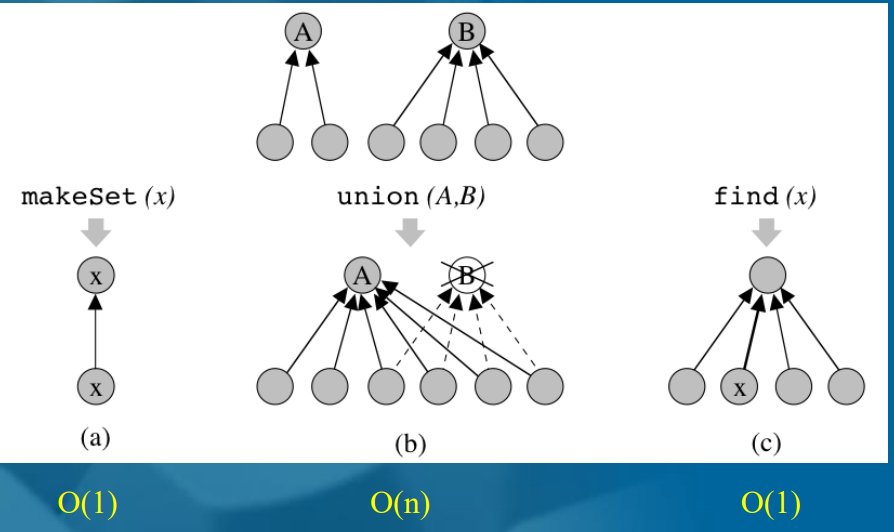
\includegraphics[width=0.5\linewidth]{QuickFind.png}
    \caption{QuickFind}
   \label{fig:enter-label}
\end{figure}

Find e makeSet richiedono solo tempo O(1), ma particolari sequenze di union possono essere molto inefficienti, $\theta (n^2)$. \newline 
Si può migliorare facendo le union in base alla grandezza degli insiemi: \newline
nell'unione degli insiemi A e B, attacchiamo gli elementi dell'insieme di cardinalità maggiore, e se necessario modifichiamo la radice dell'albero ottenuto (per aggiornare il nome). Ogni insieme mantiene esplicitamente anche la propria size (numero di elementi).
Il tempo per operazione ammortizzato sull'intera sequenza di unioni può costare $\theta(n)$, ma l'intera sequenza di n-1 union costa $O(n \log(n))$.
Vogliamo dimostrare che se eseguiamo m find, n makeset, e le al più n-1 union, il tempo richiesto dall'intera sequenza di operazioni è $O(m+n\log(n)$. L'idea della dimostrazione:
\begin{itemize}
    \item è facile vedere che find e makeSet richiedono tempo $\theta(m+n)$.
    \item Per analizzare le operazioni di union, ci concentriamo su un singolo nodo/elemento e dimostriamo che il tempo speso per tale nodo è O($\log(n)$), in totale il tempo speso è O(n$\log(n)$).
    \item Quando eseguiamo una union, per ogni nodo che cambia padre pagheremo tempo costante.
    \item Osserviamo ora che ogni nodo può cambiare al più O($\log(n)$) padri, poichè ogni volta che un nodo cambia padre la cardinalità dell'insieme cui apparteneva.
\end{itemize}
Allora il tempo speso per un singolo nodo sull'intera sequenza di n union è O($\log(n)$).
L'intera sequenza di operazioni costa O(m+n$\log(n)$).
\begin{figure}
    \centering
    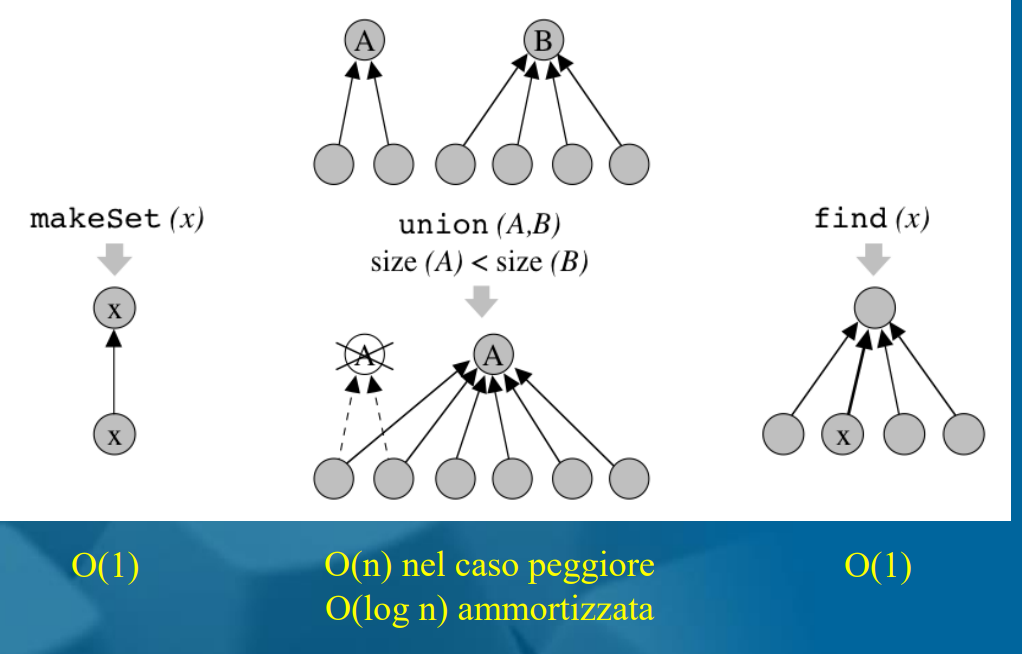
\includegraphics[width=0.5\linewidth]{quickFindBilanciato.png}
    \caption{QuickFind bilanciato}
   \label{fig:enter-label}
\end{figure}
%%%%%%%%%%%%% Algoritmo start
\begin{center}[H]
    \begin{algorithm}
        \caption{Union Find: QuickFindBilanciato implementa UnionFind}
         \SetKwData{Left}{left}\SetKwData{This}{this}\SetKwData{Up}{up}%
         \SetKwFunction{Union}{Union}\SetKwFunction{FindCompress}{FindCompress}%
         \SetKwInOut{Dati}{Dati}\SetKwInOut{Operazioni}{Operazioni}%
        \Dati{Una collezione di insiemi disgiunti di elem; ogni insieme ha un nome name.  S(n)= O(n)}
        \Operazioni{ 
     \par $-$ makeSet(elem e) crea un nuovo albero, composto da due nodi: una radice ed un unico figlio (foglia). Memorizza e sia nella foglia dell'albero che come nome nella radice. T(n) = O(1)
    
    \par $-$ union(name a, name b) Considera l'albero A corrispondente all'insieme di nome a, e l'albero B all'insieme di nome b. Se size(A) $\geq$ size(B), muovi tutti i puntatori dalle folgie di B alla radice di A, e cancella la vecchia radice di B. Altrimenti memorizza nella radice di B il nome A, muovi tutti i puntatori dalle foglie di A alla radice di B, e cancella la vecchia radice di A. In entrambi i casi assegna al nuovo insieme la somma delle cardinalità dei due insiemi originali (size(A) + size(B)).
    \par $-$ find(elem e) $\longmapsto$ name Accede alla foglia x corrispondente all'elemento e. Da tale nodo segue il puntatore al padre, che è la radice dell'albero, e restituisce il nome memorizzato in tale radice. T(n) = O(1)
        }
    \end{algorithm}
\end{center}
%%%%%%%%%%%%% Algoritmo end
\subsubsection{QuickUnion}
Per rappresentare la quickUnion useremo una foresta di alberi di altezza anche maggiore di 1 per rappresentare gli insiemi disgiunti. In ogni albero:
\begin{itemize}
    \item La radice è l'elemento rappresentativo dell'insieme;
    \item I rimanenti nodi sono gli altri elementi )escluso l'elemento nella radice).
\end{itemize}
\begin{figure}[H]
    \centering
    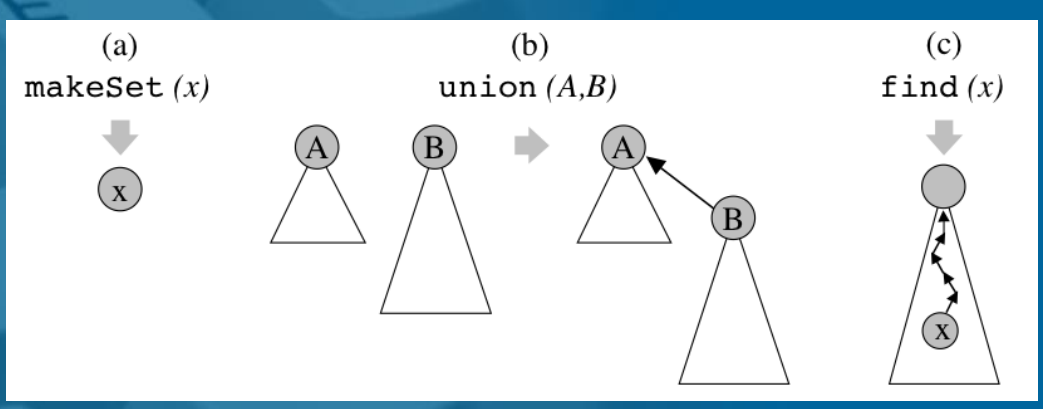
\includegraphics[width=0.5\linewidth]{quickUnion1.png}
    \caption{QuickUnion}
    \label{fig:enter-label}
\end{figure}
Eseguendo una sequenza arbitraria di operazioni, si possono generare alberi di altezza lineare, e quindi la find è molto inefficiente (costa n-1 nel caso peggiore). Quindi eseguendo n makeSet, n-1 union, seguite da m find, il tempo richiesto dall'intera sequenza di operazioni è O(mn).
Facendo la union by size, quindi unendo l'albero con la grandezza minore all'albero con la grandezza maggiore, si può  ottimizzare l'operazione di find a tempo O($\log(n)$) ottenendo O(n+m$\log(n)$) per l'intera operazione.
Questo grazie al seguente Lemma:
\begin{lemma}
    Con la union by size, dato un albero QuickUnion con size s e altezza h vale che s $\geq 2^h$.
\end{lemma}
Un'ulteriore idea, la compressione dei cammini, consiste nel comprimere il cammino (da x alla radice), ovvero rendere tutti i nodi del cammino figli della radice quando si esegue uan find(x).
\begin{theorem}
    Usando in QuickUnion le euristiche di union by size e compressione dei cammini, una qualsiasi sequenza di n makeSet, n-1 union e m find hanno un costo di O(n+m$\alpha(n+m,n)$). La funzione $\alpha(x,y)$ è detta funzione inversa della funzione di Ackermann.
\end{theorem}
La funzione di Ackermann è una funzione che cresce in modo esponenzialmente grande e veloce. La sua inversa si può definire come segue:
 $\alpha(m,n)$ = min\{i$ \geq 1 | A(i, \lfloor m/n \rfloor) > \log_{2}n$\}.
 Alcune proprietà di $\alpha(m,n)$:
 \begin{itemize}
     \item Per n fissato,  $\alpha(m,n)$ è monotonicamente decrescente al crescere di m.
     \item Per n che tende a infinito  $\alpha(m,n)$ tende a infinito.
     \item  $\alpha(m,n) \leq 4$ per ogni scopo pratico, (ovvero per valori ragionevoli di n, $n < 2^{10^{80}}$).
     \item  $\alpha(m,n) \leq 1$ quando $\lfloor m/n \rfloor > log_{2}log_{2}n$  
     \item  $\alpha(m,n) \leq 2$ quando  $\lfloor m/n \rfloor > log*log_{2}n$
 \end{itemize}
%Union-find end
%Minimum Spanning Tree start
\newpage
\subsection{Minimum Spanning Tree}
Un minimum spanning tree di un grafo G = (V, E) con pesi dei bordi a valore reale $c_e$ è un sottoinsieme di archi $T \subset E$ tali che T è uno spanning tree la cui somma dei pesi degli archi è ridotta al minimo.
\begin{theorem}
    Cayley''s Theorem: Ci sono $n^{n-2}$ spanning trees di $K_n$.
\end{theorem}
Generalmente un MST non è unico, se G ha pesi distinti allora MST è unico.
Diamo ora delle definizioni:
\begin{itemize}
    \item Cycle: insieme di archi del tipo a-b, b-c, c-d, ..., y-z, z-a.
    \item Cut: un cut è sottoinsieme di nodi S.
    \item Cutset: Un cutsed D di un cut S è un sottoinsieme di archi con esattamente un endpoint i S.
    \item Cycle-cut Intersection: Un cicloe un cutset intersecano in un nuomero pari di archi.
    \item Cut property: Sia S un qualsiasi sottoinsieme di nodi, e sia e l'arco con costo minimo con esattemente un endpoint in S. Allora esiste un MST $T^*$ che contiene e. 
    \begin{proof}
        Supponiamo che e non faccia parte di $T^*$. Aggiungiamo e a $T^*$ creando un ciclo C. Gli archi di e sono entrambi nel ciclo C e nel cutset D corrispondente a S $\Rightarrow$ Esiste un altro arco, chiamiamolo f, che sta sia in C che in D. $T' = T^*\cup \{e\} - \{f\}$ è uno spanning tree. $c_e \leq c_f, cost(T') \leq cost(T^*)$. Allora T' è un MST contentente e.
    \end{proof}
    \item Cycle property: Sia C un qualsiasi ciclo, e sia f l'arco con costo massimo dentro C. Allora esiste un MST che non contiene f.
    \begin{proof}
        Supponiamo che f appartenga a $T^*$. Cancellare f da $T^*$ creerebbe un cut S int $T^*$.
        L'arco f è sianel ciclo C che nel cutset D corrispondente a S $\Rightarrow$ esiste un altro arco, chiamiamolo e, che sta sia in C che in D. $T'=T^* \cup \{e\}-\{f\} $ è uno spanning treee. Si ha $c_e \leq c_f$, $cost(T')\leq cost (T^*)$. Allora T'' è un MST che non contiene f.
    \end{proof}
\end{itemize}
%Kruskal's algorithm start
\subsubsection{Kruskal's algorithm}
L'algoritmo di Kruskal inizia con T=$\emptyset$. Considera gli ach in ordine crescente di costo. Inserisce l'arco e in T se non crea un ciclo. Un'efficiente implementazione dell'algoritmo di Kruskal usa la  struttura dati Union-find:
\begin{itemize}
    \item per mantenere connessi tutte le componenti della soluzione corrente.
    \item Per verificare dove gli archi formano un ciclo
\end{itemize}
%%%%%%%%%% algoritmo start 
\begin{center}
\begin{algorithm}
\caption{algoritmo di Kruskal}
\KwData{grafo G=(V,e,c)}
\KwResult{albero T}
ordino gli archi in ordine crescente di costo\;
UnionFind UF\;
\For {vertice v to V}{UF.makeset(v)\;}
\For{archi (x,y) in order}
    {
    $T_x$=UF.find(x)\;
    $T_y$=UF.find(y)\;
    \If{$T_x \neq T_y$} {
        UF.union($T_x.T_y$)\;
        aggiungi  arco (x, y) a T\;
    }
    }
    \Return T\;
\end{algorithm}
\end{center}
%%%%%%%%%% algoritmo end
La correttezza dell'algoritmo è data dalla seguente osservazione: Quando si decide di aggiungere l'arco (x,y) alla soluzione poiché l'algoritmo guarda gli archi in ordine crescente di costo, l'arco con costo minimo al cut S, V\S considera il set S di vertici appartenenti alla stessa componente connessa. Quando si decide di buttare fuori un arco (x, y) dalla soluzione, poiché l'algoritmo considera gli archi in ordine crescente di costo, l'arco di costo massimo che forma il ciclo resta fuori dalla soluzione. (?????? approfondire)
Il costo computazionale dall'algoritmo è $O(m \log n +UF(m,n))$ visto che ci sono n makeset, n-1 union, m find. Se si usa la quickFind si ottine $O(m \log n +n \log n)$, con la quickUnion $O(m \log n +m \log n +n)$, in entrambi i casi si ha $O(m \log n)$.
%Kruskal's algorithm end
%algoritmo di Prim start
\subsubsection{Prim's algorithm}
L'algoritmo di Prim inizia da un qualsiasi nodo radice s e in modo greedy aggiunge nodi all'albero T da s verso l'esterno. Ad ogni step, aggiunge l'arco di costo minore a T che ha esattamente un endpoint in T. La correttezza è data dalla cut property usata esattamente n-1 volte.
Il costo computazionale dell'algoritmo di Prim è O(mn), perchè per n-1 volte si cerca un arco di costo minimo nel cut introdotto dall'albero parziale in tempo O(m).
Un'implementazione più veloce implica Mantenere un set di nodi esplorati S, usare una priority queue per mantenere i nodi non esplorati. 
%%%%%%%%%% algoritmo start 
\begin{center}
\begin{algorithm}
\caption{algoritmo di Prim}
\KwData{grafo G=(V,e,c), nodo s}
\KwResult{albero T}
\For {vertice v to V}{a[v]$\leftarrow \infty$ \;}
a[s] $\leftarrow 0$\;
Q priority queue\;
\For {vertice v to V}{inserisci v in Q con priorità a[v]}
\While{Q is not empty}{
    u $\leftarrow$cancella l'elemento con costo minimo da Q\;
    S $\leftarrow S \cup \{u\}$\;
    \For{arco e = (u,v) incidente a u}{
        \If{$(v \notin S) and (c_e < a[v]$}{
            setta u parente di v in T\;
            decrementa a[v] di $c_e$ nella priority queue\;
        }
    }
}
\Return T\;
\end{algorithm}
\end{center}
%%%%%%%%%% algoritmo end
Il costo computazionale è:
\begin{itemize}
    \item O(m+n) costo delle operazioni della priority queue;
    \item n insert, n delete min, m decrease key.
    \item O($n^2$) con gli array; O($m \log n$) con gli heap binari;
    \item O(m+ $n \log n$) con gli heap di Fibonacci.
\end{itemize}
%algoritmo di Prim end
%Clustering start
\subsubsection{Clustering}
Verificare se va fatto
%Clustering end
%Minimum Spanning Tree end
%Algoritmi Greedy end
%Programmazione Dinamica start
\section{Programmazione Dinamica}
%Insieme Indipendente di peso massimo start
\subsection{Insieme Indipendente di peso massimo (su grafi a commino)}
Dato in input un cammmino G di n nodi. Ogni nodo $v_i$ ha un peso $w_i$. L'obiettivo è trovare un insieme indipendente di peso massimo, ovvero un insieme S di nodi tale che: 
\begin{itemize}
    \item S è un II,
    \item w(S)=$\sum_{v_i \in S}w_i$ è più grande possibile.
\end{itemize}
L'idea è di enumerare tutti i sottiinsiemi degli n nodi, per ognuno verifichiamo che è un insieme indipendente, ne calcoliamo il peso e teniamo quello di peso massimo. Con un approccio greedy non si riesce a costruire un algoritmo corretto, con il divide et impera risulta molto complesso trovare un algoritmo corretto, allora bisogna cambiare approccio e sfruttare le tecniche di programmazione dinamica. L'idea è ragionare sulla struttura/proprietà della soluzione (ottima) del problema, in termini di soluzioni ottime di sottoproblemi più piccoli, similmente a come si fa con la tecnica del divide-et-impera. L'obiettivo è esprimere la soluzione del problema come combinazioni di soluzioni di opportuni sotto problemi. Se le combinazioni sono poche, si può cercare la combinazione giusta per forza bruta.
Sia $S^*$ la soluzione ottima, ovvero l'insieme indipendente di peso massimo di G. Consideriamo l'ultimo nodo di G, $v_n$. Allora o $v_n \in S^*$ oppure $v_n \notin S^*$:
\begin{itemize}
    \item $v_n \notin S^*$: considera $G'=G-\{v_n\}$. Allora $S^*$ è una soluzione ottima per G'. Se esistesse una soluzione S migliore per G', S sarebbe migliore anche per G: assurdo!
    \item $v_n \in S^*$: considera $G''=G-\{v_{n-1}, v_n\}$. Allora $S^*\ \{v_n\}$ è una soluzione ottima per G''. Se esistesse una soluzione S migliore per G'', S$\cup\{v_n\}$ sarebbe migliore di S* per G: assurdo! 
\end{itemize}
Proprietà: l'II di peso massimo per G deve essere o l'II di peso massimo per G', o $v_n$ unito all'II di peso massimo per G''. L'idea è di procedere iterativamente considerando prefissi di G dai più piccoli verso i più grandi. 
Sia $G_j$ il sottocammino composto dai primi j vertici di G; OPT[]: vettore di n elementi; dentro OPT[j] vogliamo mettere il peso dell'II di peso massimo $G_j$.
%%%%%%%%%% algoritmo start 
\begin{center}
\begin{algorithm}
\caption{valore della soluzione ottima}
\KwData{$w_1,\dots,w_n$}
\KwResult{int value}
OPT[1]=$w_1$\;OPT[2]=max{$w_1,w_2$}\;
\For {j=3 to n}{OPT[j]=max$\{OPT[j-1], w_j+OPT[j-2]\}$\;}
\Return OPT[n]\;
\end{algorithm}
\end{center}
%%%%%%%%%% algoritmo end
Per ricostruire la soluzione, si può sfruttare il vettore OPT[] usando la seguente proprietà:
$v_j \in II$ di peso massimo di $G_j \Leftrightarrow w_j + OPT[j-2] \geq OPT[j-1]$.
%%%%%%%%%% algoritmo start 
\begin{center}
\begin{algorithm}
\caption{Ricostruiamo la soluzione ottima}
\KwData{$w_1,\dots,w_n$}
\KwResult{Array}
S=$\emptyset$\;j=n\;
\While {j$\geq 3$}{
\If{OPT[j-1]$\geq w_j + OPT[j-2]\;$}{j=j-1\;}
\Else{$S^*=S^*\cup\{v_j\}\;$j=j-2\;}
}
\If{j=2 and $ w_2 > w_1$}{$S^*=S^*\cup\{v_2\}\;$}
\Else{$S^*=S^*\cup\{v_1\}\;$}
\Return $S^*$\;
\end{algorithm}
\end{center}
%%%%%%%%%% algoritmo end
%Insieme Indipendente di peso massimo end
%principi generali start
\subsection{Programmazione Dinamica: principi generali}
\begin{itemize}
    \item Identificare un numero piccolo di sottoproblemi;
    \item Descrivere la soluzione di un generico sottoproblema in funzione delle soluzioni di sottoproblemi più piccoli;
    \item Le soluzioni dei sottoproblemi sono memorizzate in una tabella;
    \item Avanzare opportunamente sulla tabella, calcolando la soluzione del sottoproblema corrente in funzione delle soluzioni di sottoproblemi già risolti.
\end{itemize}
Proprietà che devono avere i sottoproblemi:
\begin{itemize}
    \item Essere pochi;
    \item Risolti tutti i sottoproblemi si può calcolare velocemente la soluzione al problema originale;
    \item Ci devono essere sottoproblemi piccoli
    \item Ci deve essere un ordine in cui risolvere i sottoproblemi
\end{itemize}
%principi generali end
%Weighted interval scheduling start
\subsection{Weighted interval scheduling}
Dati degli intervalli del tipo, intervallo j [$s_j,f_j$] con larghezza $w_j>0$, due intervalli sono compatibili se non si sovrappongono, trovare il sottoinsieme di intervalli mutualmente compatibili di larghezza massima.
Una prima idea per risolvere questo algoritmo, potrebbe essere quella di risolverlo con il metodo greedy usando l'earliest-finish-time, ma questo è corretto solo se tutte le larghezze sono 1.
Siano gli intervalli ordinati per finish time: $f_1 \leq f_2 \leq \dots \leq f_n$.
Sia p(j) il più largo indice tale che un intervallo i sia compatibile con j.
Definiamo OPT(j) come la massima larghezza di ogni sottoinsieme di intervalli mutualmente esclusivi costituito dai sottoinsiemi 1, 2, ..., j.
L'obiettivo è trovare OPT(n), la massima larghezza di ogni sottoinsieme con intervalli compatibili.
Ci sono due casi:
\begin{itemize}
    \item OPT(j) non seleziona j, si ha che la soluzione ottima contiene gli intervalli 1, 2, ...,j-1.
    \item OPT(j) seleziona j: aggiunge alla soluzione $w_j$, non può considerare gli intervalli non compatibili {p(j)+1,p(j)+2,...,j-1}. Deve includere la soluzione ottimale del problema degli intervalli 1, 2, ..., p(j).   
\end{itemize}
Equazione di Bellman: 
\[
OPT(j) =\begin{cases} 0, & \mbox{se }j=0 \\ max\{OPT(j-1), w_j+OPT(p(j))\}, & \mbox{se }j>0
\end{cases}
\]
Abbiamo due modi per risolvere questo problema, usando la bottom-up dynamic programming (Table-based) o la top-down programming (memoization).
%bottom-up dynamic programming start
\subsubsection{Bottom-up dynamic programming}
%%%%%%%%%% algoritmo start 
\begin{center}
\begin{algorithm}
\caption{Bottom-up}
\KwData{$n,s_1,\dots,s_n,f_1,\dots,f_n,w_1,\dots,w_n$}
\KwResult{int}
Ordino gli intervalli per finish time e li rinomino in modo opportuno, $f_1 \leq f_2 \leq \dots \leq f_n$\;
Calcolo p[1],p[2],...,p[n] con la ricerca binaria\;
M[0]$\leftarrow$0\;

\For {j=1 to n}{
    $M[j]\leftarrow max\{M[j-1],w_j+M[p[j]]\}$
}
\Return $M[n]$\;
\end{algorithm}
\end{center}
%%%%%%%%%% algoritmo end
Questa versione del bottom-up ha costo computazionale $O(n \log n)$. L'ordinamento costa $O(n \log n)$ usando il mergesort, il calcolo p[j] per ogni j costa $O(n \log n)$ con la ricerca binaria, il ciclo for O(n).
Ecco una versione ricorsiva dell'algoritmo:
%%%%%%%%%% algoritmo start 
\begin{center}
\begin{algorithm}
\caption{Bottom-up}
\KwData{$n,s_1,\dots,s_n,f_1,\dots,f_n,w_1,\dots,w_n$}
\KwResult{int}
Ordino gli intervalli per finish time e li rinomino in modo opportuno, $f_1 \leq f_2 \leq \dots \leq f_n$\;
Calcolo p[1],p[2],...,p[n] con la ricerca binaria\;
\Return $Compute-OPT(n)$\;
\end{algorithm}
\end{center}
%%%%%%%%%% algoritmo end
%%%%%%%%%% algoritmo start 
\begin{center}
\begin{algorithm}
\caption{Compute-OPT}
\KwData{$j$}
\KwResult{int}
\If{j = 0}{\Return 0\;}\Else{
\Return $max\{Compute-OPT(j-1),w_j+Compute-OPT(p[j])\}$\;}
\end{algorithm}
\end{center}
%%%%%%%%%% algoritmo end
Osservazione: L'algoritmo ricorsivo è più lento per via dei numerosi sottoproblemi, ha un costo computazionale esponenziale.
%bottom-up dynamic programming end
%top-down dynamic programming start
\subsubsection{Top-down dynamic programming}
%%%%%%%%%% algoritmo start 
\begin{center}
\begin{algorithm}
\caption{Top-Down}
\KwData{$n,s_1,\dots,s_n,f_1,\dots,f_n,w_1,\dots,w_n$}
\KwResult{int}
Ordino gli intervalli per finish time e li rinomino in modo opportuno, $f_1 \leq f_2 \leq \dots \leq f_n$\;
Calcolo p[1],p[2],...,p[n] con la ricerca binaria\;
M[0]$\leftarrow0 \leftarrow $array globale\;
\Return $M-Compute-Opt(n)$\;
\end{algorithm}
\end{center}
%%%%%%%%%% algoritmo end
%%%%%%%%%% algoritmo start 
\begin{center}
\begin{algorithm}
\caption{M-Compute-Opt}
\KwData{$j$}
\KwResult{int}
\If{M[j] non è inizializzato}{
M[j]$\leftarrow max\{M-Compute_Opt(j-1),w_j+M-Compute_Opt(p[j])\}$\;
}
\Return M[j]\;
\end{algorithm}
\end{center}
%%%%%%%%%% algoritmo end
Questo algoritmo ha costo computazionale O(n$\log n$).
\begin{proof}
    L'ordinamento ha costo $O(n \log n)$ via mergesort. Calcolare p[j] per ogni j costa $O(n \log n)$ via ricerca binaria.
    M-Compute-Opt ogni invocazione costa O(1), e per ognuna o torna un array inizializzato, o inizializza M[j] e crea due chiamate ricorsive.
    Sia $\phi$ il numero di voci inizializzate tra M[1 ... n]. Inizialmente $\phi$ = 0; Finchè $\phi$ < 0, incrementiamo $\phi$  di 1 per ogni chiamata ricorsiva, allora ci saranno $\leq 2n$ chiamata ricorsive. Il costo computazionale di M-Compute-Opt(n) allora è O(n).
\end{proof}
%top-down dynamic programming end
Questi algoritmo calcolano il valore ottimo, per trovare la soluzione ottima dobbiamo procedere come segue:
%%%%%%%%%% algoritmo start 
\begin{center}
\begin{algorithm}
\caption{Find-Solution}
\KwData{$j$}
\KwResult{[]}
\If{j=0}{
\Return $\emptyset$\;
}
\If{$w_j + M[p[j]] > M[j-1]$}{
\Return {j}$\cup$ Find-Solution(p[j])\;
}
\Return Find-Solution(j-1)\;
\end{algorithm}
\end{center}
%%%%%%%%%% algoritmo end
Il numero di chiamate ricorsive di questo algoritmo è $\leq n \Rightarrow O(n)$.
\subsubsection{ top-down vs bottom-up}
Top-down (Memoization):
\begin{itemize}
    \item L'approccio Top-down è più intuitivo;
    \item Indicizzare i sottoproblemi è più semplice (esempio insiemi).
    \item Calcola solo i sottoproblemi necessari.
    \item Le chiamate di funzione overhead (????)
    \item Il costo computazionale è difficile da analizzare
\end{itemize}
Bottom-Up(Table-based):
\begin{itemize}
    \item  Più difficile da comprendere
    \item Necessita di indicizzare i sottoproblemi con numeri interi.
    \item Calcola sempre tutti i sottoproblemi.
    \item No ricorsione, cache più efficiente.
    \item Il costo computazionale è più semplice da analizzare.
    \item Codice più corto e pulito.
\end{itemize}
%Weighted interval scheduling end
%Longest Increasing Subsequence start
\subsection{Longest Increasing Subsequence}
Data una sequenza di elementi ordinabili, trovare la più lunga sotto sequenza di elementi ordinati in ordine crescente.\newline
Definizione del sottoproblema: OPT[i] è la lunghezza del Longest Increasing Subsequence di S[1], ..., S[i] che finisce per S[i].\newline
Caso base OPT[1] = 1.\newline
Soluzione: $max_{i=1,2,\dots,n}OPT[i]$; l'ordine dei sottoproblemi è OPT[1], ..., OPT[n].\newline
La formula ricorsiva è la sequente: OPT[i]=1+max$\{0,max_{j=1,2,\dots,i-1 t.c. S[j]<S[i]}OPT[j]\}$.
%%%%%%%%%% algoritmo start 
\begin{center}
\begin{algorithm}
\caption{LIS}
\KwData{$S[1:n]$}
\KwResult{int}
$OPT[1]\leftarrow1\;$
\For{i=2 to n}{
OPT[i]=1+max$\{0,max_{j=1,2,\dots,i-1 taleche S[j]<S[i]}OPT[j]\}$\;
}
\Return $max_i OPT[i]$\;
\end{algorithm}
\end{center}
%%%%%%%%%% algoritmo end
Il costo compitazionale dell'algoritmo è O($n^2$) visto che ogni OPT[i] viene calcoltato O(i)=O(n) volte.
%Longest Increasing Subsequence end
%House Coloring problem start
\subsubsection{House coloring problem}
Dipingi una riga di n case rosse, verdi o blu in modo tale che:
\begin{itemize}
    \item Non ci siano due case adiacenti aventi lo stesso colore;
    \item Minimizzi il costo, dove costo(i,color) è il costo di dipingere i del colore color.
\end{itemize}
Sottoproblemi:
\begin{itemize}
    \item R[i]= minimo il costo di dipingere le case 1,...,i con i rossi.
    \item G[i]= minimo il costo di dipingere le case 1,...,i con i green.
    \item B[i]= minimo il costo di dipingere le case 1,...,i con i blue.
\end{itemize}
Costo ottimo = min {R[n],G[n],B[n]}.\newline
Equazione:
\begin{itemize}
    \item R[i]=cost(i,red) + min{B[i-1],G[i-1]}.
    \item G[i]=cost(i,green) + min{R[i-1],B[i-1]}.
    \item B[i]=cost(i,blue) + min{R[i-1],G[i-1]}.
\end{itemize}
Costo computazionale: O(n).
trovare l'algoritmo!!!
%House Coloring problem end
%Segmented least square start
\subsection{Segmented least squares}
Dati n punti in un piano: $(x_1,y_1), (x_2,y_2), \dots, (x_n,y_n)$, trovare una retta y=ax+b che minimizzi la somma dell'errore quadratico: 
\begin{center}
    SSE=$\sum_{i=1}^n(y_i-ax_i-b)^2$. 
\end{center}
Questo accade quando:
\begin{center}
    a=$\dfrac{n\sum_ix_iy_i-(\sum_ix_i)(\sum_iy_i)}{n\sum_ix_i^2-(\sum_ix_i)^2}$
    b=$\dfrac{\sum_iy_i-a\sum_ix_i}{n}$
\end{center}
L'obiettivo è quindi minimizzare $f(x)=E+cL$ per qualche c>0, dove:
\begin{itemize}
    \item E = somma delle summe degli errori quadratici per ogni segmento.
    \item numero di linee.
\end{itemize}
Avremo quindi OPT(j) = minimo costo per i punti $p_1,\dots,p_j$ e $e_{ij}=$SSE per i punti $p_i,p_{i+1},\dots,p_j$.\\ 
Bellman equation:\\
\[
OPT(j) =\begin{cases} 0, & \mbox{se }j=0 \\ min_{1\leq i \leq j}\{r_{ij}+c+OPT(i-1)\}, & \mbox{se }j>0
\end{cases}
\]
%%%%%%%%%% algoritmo start 
\begin{center}
\begin{algorithm}
\caption{Segmented-least-squares}
\KwData{$n,p_1,\dots,p_n,c$}
\KwResult{int}
\For{i=1 to n}{
    \For{i=1 to j}{
        Calcola SSE $e_{ij}$ per i punti $p_1,p_{i+1},\dots,p_j$.   
    }
}
M[0]$\leftarrow$0.
\For{j=1 to n}{
M[j]$\leftarrow min_{\ \leq i \leq j}\{e_{ij}+c+M[i-1]\}$
}
\Return $M[n]$\;
\end{algorithm}
\end{center}
%%%%%%%%%% algoritmo end
Questo algoritmo risolve il segmented least squares problem in temo $O(n^3)$ e con spazio $O(n^2)$.\\
\begin{proof}
    Bottleneck = calcolo SSE $e_{ij}$ per ogni i e j.\\
    \begin{center}
    a=$\dfrac{n\sum_kx_ky_k-(\sum_kx_k)(\sum_ky_k)}{n\sum_kx_k^2-(\sum_kx_k)^2}$
    b=$\dfrac{\sum_ky_k-a_{ij}\sum_kx_k}{n}$
    \end{center}
    Tempo di calcolo di $e_{ij}$ è O(n).
\end{proof}
Può essere sviluppato in tempo $O(n^2)$.\\ Per ogni i: mi precalcolo le somme $\sum_k=1^ix_k, \sum_k=1^iy_k, \sum_k=1^ix_k^2, \sum_k=1^ix_ky_k$. Usando queste somme precalcolate, calcolo $e_ij$ in tempo costante.
%Segmented least square end
%knapsack problem start
\subsection{knapsack problem}
Il goal è di massimizzare il totale dei valori degli oggetti "messi nello zaino".
\begin{itemize}
    \item Ci sono n oggetti: l'iesimo oggetto ha valore $v_i>0$ e occupa $w_i>0$ spazio.
    \item Il valore di un sottoinsieme di oggetti è la somma dei valori degli oggetti singoli.
    \item Lo zaino ha spazio limite W.
\end{itemize}
Si assuma che i valori degli oggetti e lo spazio che occupano siano interi.\\
Sia OPT(i) = il valore ottimo del problema con gli oggetti 1, ..., i.
Ci sono due casi:
\begin{itemize}
    \item OPT(i) non selezione l'i-esimo oggetto, selezionerà quindi l'ottimo tra {1, 2, ...,i-1}.
    \item OPT(i) seleziona l'i-esimo oggetto. Selezionare l'i-esimo oggetto non implica che aggiamo rifiutato gli altri oggetti, senza sapere quali altri oggetti abbiamo selezionato prima di i, non possiamo sapere se abbiamo abbastanza spazio per i. Vanno quindi definiti dei sottoproblemi.
\end{itemize}
Sia OPT(i,w) il valore ottimo per gli oggetti 1, ..., i, con limite di spazio w. 
Ci sono due casi:
\begin{itemize}
    \item OPT(i) non selezione l'i-esimo oggetto, selezionerà quindi l'ottimo tra {1, 2, ...,i-1} con limite di spazio w.
    \item OPT(i) seleziona l'i-esimo oggetto, il nuovo spazio limite sarà $w - w_i$. Il valore OPT(i,w) sarà il migliore tra {1, 2, ..., i-1} con il nuovo limite.
\end{itemize}
Bellman equation:\\
\[
OPT(i, w) =\begin{cases} 0, & \mbox{se }i=0 \\ OPT(i-1,w), & \mbox{se }w_i>w \\ max\{OPT(i-1,w),v_i+OPT(i-1,w-w_i)\} & \mbox{altrimenti }
\end{cases}
\]
%%%%%%%%%% algoritmo start 
\begin{center}
\begin{algorithm}
\caption{Knapsack}
\KwData{$n,W,w_1,\dots,w_n,v_1,\dots,v_n$}
\KwResult{int}
\For{w=0 to W}{
  M[0,w]$\leftarrow0.$
}
\For{i=1 to n}{
    \For{w=0 to W}{
        \If{$w_i>i$}{
            M[i-1,w]$\leftarrow$ M[i-1,w].
        }
        \Else{
            M[i, w]$\leftarrow$ max$\{M[i-1, w], v_i + M[i-1,w-w_i]\}$.
        }
    }
}
\Return $M[n,W]$\;
\end{algorithm}
\end{center}
%%%%%%%%%% algoritmo end
\begin{theorem}
    Questo algoritmo risolve il problema del Knapsack con n oggetti e spazio massimo W con tempo $\theta(nW)$ e spazio $\theta(nW)$.
\end{theorem}
\begin{proof}
    \begin{itemize}
        \item Ogni elemento aggiunto alla matrice costa O(1).
        \item Ci sono $\theta (nW)$ elementi nella matrice
        \item Sopo aver calcolato i valori ottimi, si può fare backtrack per trovare la soluzione: OPT(i,w) prende l'oggetto i se M[i,w]>M[i-1,w].
    \end{itemize}
\end{proof}
L'algoritmo dipende dal fatto che abbiamo assunto lo spazio intero, non dipende dal tipo usato per i valori.\\
Questo algoritmo non è polinomiale perché $\theta (nW)$ non è una funzione polinomiale rispetto all'input. Si definisce pseudo polinomiale.\\
Un algoritmo si definisce pseudo polinomiale quando è polinomiale nei valori dell'input: """"""verificare""""""""
\begin{itemize}
    \item Efficiente quando i numeri coinvolti nell'input sono ragionevolmente piccoli
    \item Non necessariamente polinomiale nella dimensione dell'input.
\end{itemize}
%knapsack problem end
%Sequence alignment start
\subsection{Sequence alignment}
Questo problema punta a verificare quanto due stringhe siano simili. Per far ci; va definita la edit distance:
\begin{itemize}
    \item Gap penalty $\delta$; mismatch penalty $\alpha_{pq}$.
    \item Cost = somma dei gap e mismatch penalty.
\end{itemize}
Il problema può essere definito come segue: date due stringhe $x_1 x_2 \dots x_m$ e $y_1 y_2 \dots y_n$ trovare l'allineamento con costo minore.\\
Un allinemamento M è un set di coppie ordinate $x_i - y_j$ che ogni carattere appare al massimo in una coppia e senza incroci. Il costo dell'allinemamento M è:
\begin{center}
    cost(M) = $\sum_{(x_i,y_j)\in M}\alpha_{x_iy_j}+\sum_{i:x_i unmatch}\delta + \sum_{j:y_j unmatch}\delta$
\end{center}
Definiamo OPT(i,j)= allineamento di costo minimo delle stringhe $x_1 x_2 \dots x_i$ e $y_1 y_2 \dots y_j$.L'obiettivo è trovare OPT(m,n).\\
Ci sono vari casi:
\begin{itemize}
    \item OPT(i,j) corrisponde a $x_i-y_j$. Costa il mismatch per $x_i-y_j$ + l'allineamento dal costo minimo tra $x_1 x_2 \dots x_{i-1}$ e $y_1 y_2 \dots y_{j-1}$.
    \item OPT(i,j) lascia $x_i$ senza corrispondenza. Costa il gap per $x_i$+ l'allineamento dal costo minimo tra $x_1 x_2 \dots x_{i-1}$ e $y_1 y_2 \dots y_{j}$.
    \item OPT(i,j) lascia $y_i$ senza corrispondenza. Costa il gap per $y_i$+ l'allineamento dal costo minimo tra $x_1 x_2 \dots x_{i}$ e $y_1 y_2 \dots y_{j-1}$.
\end{itemize}
Bellman equation:\\
\[
OPT(i, j) =\begin{cases} j\delta, & \mbox{se }i=0 \\ i\delta, & \mbox{se }j=0 \\ min\begin{cases}
    \alpha_{x_iy_i}+OPT(i-1,j-1)\\ \delta + OPT(i-1,j) \\ \delta + OPT(i,j-1)
\end{cases} & \mbox{altrimenti }
\end{cases}
\]
%%%%%%%%%% algoritmo start 
\begin{center}
\begin{algorithm}
\caption{Sequence-alignment}
\KwData{$m,n,x_1,\dots,x_m,y_1,\dots,y_n,\delta,\alpha$}
\KwResult{int}
\For{i=0 to m}{
  M[0,j]$\leftarrow i\delta.$
}
\For{j=0 to n}{
  M[0,j]$\leftarrow j\delta.$
}
\For{i=1 to m}{
    \For{j=1 to n}{
        M[i,j]$\leftarrow min\{\alpha_{x_iy_i}+M[i-1,j-1],\delta + M[i-1,j], \delta + M[i,j-1]\}\;$
    }
}
\Return $M[m, n]$\;
\end{algorithm}
\end{center}
%%%%%%%%%% algoritmo end
\begin{theorem}
    Questo algoritmo, con due stringhe di m e n caratteri calcola la edit distance (e l'allineamento ottimale) in tempo e spazio $\theta(mn)$.
\end{theorem}
\begin{proof}
    L'algoritmo calcola la edit distance. Si può fare backtracking per estrarre l'allineamento ottimale stesso.
\end{proof}
%Sequence alignment end
%Algoritmo di Hirschberg start
\subsection{Algoritmo di Hirschberg}
Esiste un algoritmo per trovare un allineamento ottimale in tempo O(mn) e spazio O(m+n) che sfrutta un'intelligente combinazione del divide-et-impera e della programmazione dinamica.\\
Visto che per calcolare la prossima colonna/riga della matrice abbiamo bisogno solo della precedente colonna/riga, allora manteniamo solo 2 colonne/righe alla volta e lo spazio richiesto per questo è O(m+n). Questo permette di calcolare la edit distance, ma non l'allineamento. Definiamo ora il grafo per la edit distance.\\
\begin{figure}[H]
    \centering
    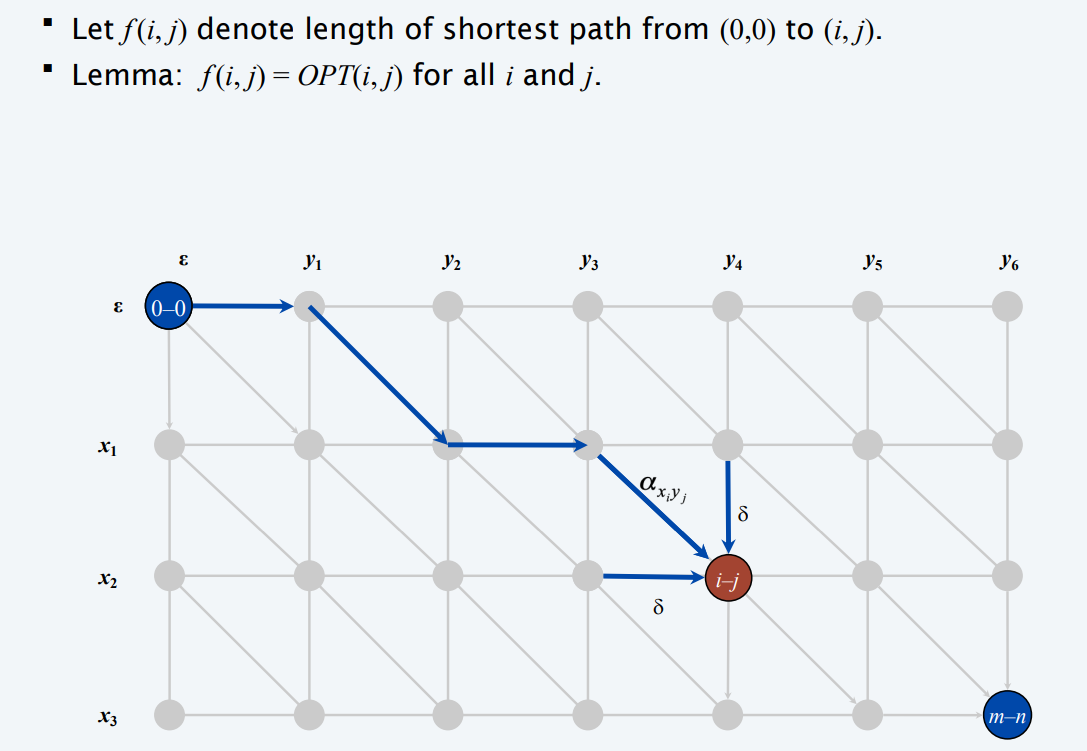
\includegraphics[width=0.5\linewidth]{hirschberg.png}
    \caption{Edit distance graph 2}
    \label{fig:enter-label}
\end{figure}
\begin{lemma}
    f(i,j)=OPT(i,j) per ogni i e j.
\end{lemma}
\begin{proof}
    Caso base: f(0,0)=OPT(0,0)=0.
    Ipotesi induttiva: assumiamo vero per ogni (i',j') con i'+j'<i+j. L'ultimo arco sul percorso più breve verso (i,j) proviene da (i-1,j-1), (i-1,j) o (i, j-1). Così,\\
    f(i,j)=$min\{\alpha_{x_iy_i}+f(i-1, j-1), \delta+f(i-1,j), \delta+f(i,j-1)\}\\=min\{\alpha_{x_iy_i}+OPT(i-1, j-1), \delta+OPT(i-1,j), \delta+OPT(i,j-1)\}\\=OPT(i,j)$
\end{proof}
Si può calcolare f(*,j) per ogni j in tempo O(mn) e spazio O(m+n). Sia g(i,j) la lunghezza del percorso più corto da (i,j) a (m,n). Si può calcolare g(i,j) invertendo l'orientamento degli archi e invertendo i ruoli di (0,0) e (m,n).
\begin{figure} [H]
    \centering
    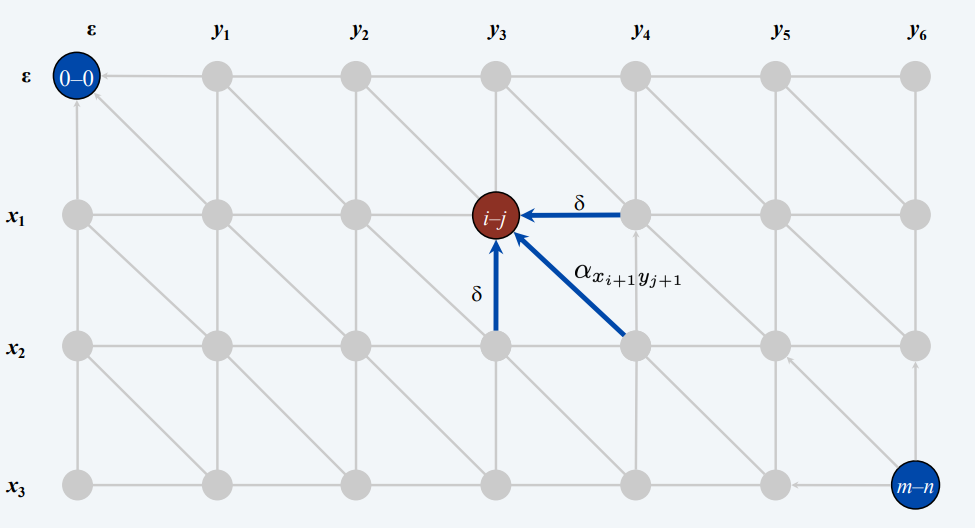
\includegraphics[width=0.5\linewidth]{hirschberg1.png}
    \caption{Edit distance graph 2}
    \label{fig:enter-label}
\end{figure}
Osservazioni:
\begin{itemize}
    \item La lunghezza del più corto path che usa (i,j) è f(i,j)+g(i,j).
    \item Sia q un indice che minimizza f(1,n/2)+g(q,n/2). Allora esiste uno shortest path da (0,0) a (m,n) che usa (q,n/2).
\end{itemize}
Divede-et-impare: Divide trova l'indice q che minimizza f(1,n/2)+g(q,n/2); salvare il nodo (i,j) come parte della soluzione. Impera, ricorsivamente calcola l'allineamento ottimo in ogni pezzo.
\begin{figure}[H]
    \centering
    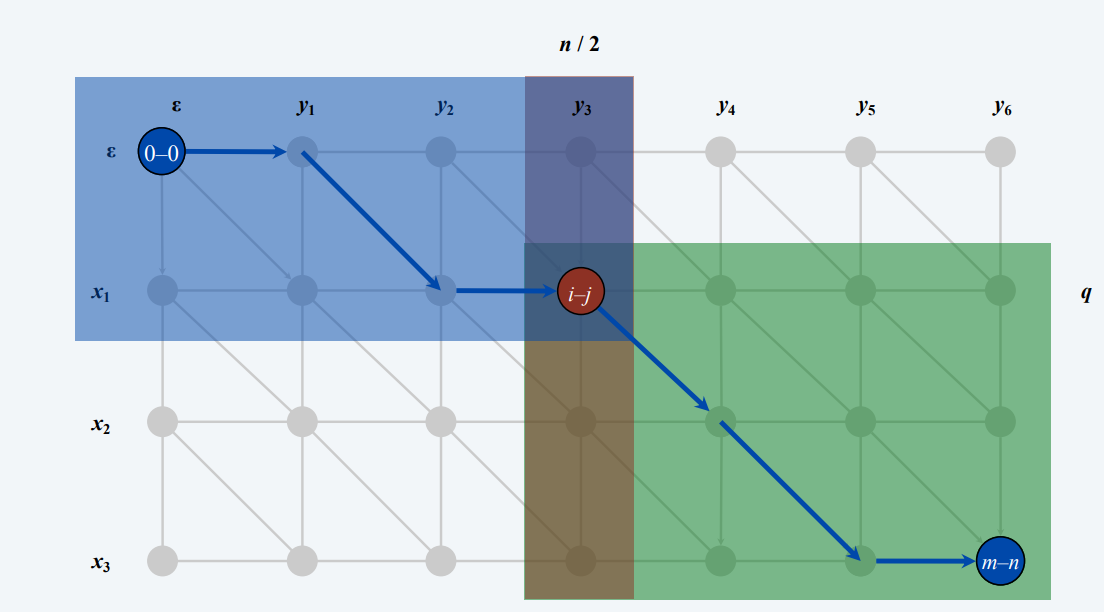
\includegraphics[width=0.5\linewidth]{hirschbergDivEtImp.png}
    \caption{Divide et impera}
    \label{fig:enter-label}
\end{figure}
\begin{theorem}
    L'algoritmo di Hirschberg usa spazion $\theta(m+n)$.
\end{theorem}
\begin{proof}
    Ogni chiamata ricorsiva usa spazio $\theta(m)$ per calcolare f(*,n/2) e g(*,n/2). Per ogni chiamata ricorsiva è necessario mantenere spazio costante, il numero di chiamate ricorsive è $\leq n$.
\end{proof}
\begin{theorem}
    Sia T(m,n)= il tempo massimo di esecuzione di questo algoritmo su stringhe di lunghezza m e n. Allora, T(m,n)=O(mn).
\end{theorem}
\begin{proof}
    \begin{itemize}
        \item O(mn) è il tempo per calcolare f(*,n/2) e g(*,n/2) e trovare l'indice q.
        \item T(q,n/2)+T(m-q,n/2) il tempo per due chiamate ricorsive.
        \item Trovare una costante c tale che: T(m,2)$\leq cm \leq cn \leq cmn+T(q,n/2)+T(m-q,n/2)$
        \item T(m, n) $\leq$ 2cmn.
        \item Caso base: m=2, n=2.
        \item Iportesi induttiva: T(m',n')$\leq 2cm'n'$ per ogni (m',n') con m'+n' < m+n.\\
        T(m,n)$\leq T(q,n/2)+T(m-q,n/2)+cmn\\ \leq 2cqn/2 + 2c(m-q)n/2 +cmn\\ =cqn+cmn-cqn-cmn\\ =2cmn$
    \end{itemize}
\end{proof}
%Algoritmo di Hirschberg end
%Bellman–Ford–Moore algorithm start
\subsection{Bellman–Ford–Moore algorithm}
Sia G=(V,E) un grafo diretto con lunghezza degli archi arbitrale $l{vw}$, trovare lo shortest path dal nodo sorgente s al destinatario t.\\
Note:
\begin{itemize}
    \item Non si può produrre uno shortest path se la lunghezza dei lati è negativa.
    \item L'aggiunta di una costante ad ogni lunghezza dell'arco non fa si che l'algoritmo di Dijkstra produca lo shortest path.
    \item Un ciclo negativo è un cyclo tale che l(W)=$\sum l_e<0$.
\end{itemize}
\begin{lemma}
    Se qualche path(v,t) contiene un ciclo negativo, allora non esiste uno shortest path(v,t).
\end{lemma}
\begin{proof}
    Se esiste un ciclo W, allora possiamo costruire un path(v,t) di lunghezza negativa arbitraria deviando attorno a W quante volte si desidera.
\end{proof}
\begin{lemma}
    Se G non ha cicli negativi, allora esiste uno shortest part(v,t) che sia più piccolo e che abbia $\leq n-1$ archi.
\end{lemma}
\begin{proof}
    Tra tutti i path(v,t) più brevi, considera quello che utilizza il minor numero di archi. Se il path P contiene un ciclo diretto W, allora si può rimuovere una porsione di P corrispondende a W senza incrementare la lunghezza
\end{proof}
%Single-destination shortest-paths problem start
\subsubsection{Single-destination shortest-paths problem}
Sia G=(V,E) con lunghezza archi negativa $l_{vw}$ e sia t un nodo distinto, trovare uno shortest path(v,t) per ogni nodo v.\\
Negative-cycle problem:\\
Sia G=(V,E) un grafo diretto con lunghezza $l_{vw}$, trovare un ciclo negativo (se esiste).\\
Definiamo OPT(i,v) come la lunghezza dello shortest path(v,t) che usa $\leq i$ lati. L'obiettivo è trovare OPT(n-1,v) per ogni v.
Ci sono due casi:
\begin{itemize}
    \item Lo shortest path(v,t) usa $\leq$ i-1 archi. OPT(i,v)=OPT(i-1,v).
    \item Lo shortest path(v,t) usa esattamente i archi. Se (v,w) è il primo arco dello shortest apth(v,t), il costo è $l_{vw}$. Altrimenti, seleziono l'ottimo usando $\leq$i-1 archi.
\end{itemize}
Bellman equation:\\
\[
OPT(i, v) =\begin{cases} 0, & \mbox{se i=0 and }v=t \\ \infty, & \mbox{se i=0 and }v \neq t \\ min\{OPT(i-1,v), min\{OPT(i-1,w)+l_{vw}\}\}& \mbox{se }i  > 0 
\end{cases}
\]
%%%%%%%%%% algoritmo start 
\begin{center}
\begin{algorithm}
\caption{Shortest-Path with negative wights}
\KwData{$V,E,l,t$}
\For{node v $\in$V}{
  M[0,j]$\leftarrow\infty\;$
}
\For{i=0 to n-1}{
    \For{node v$\in$V}{
        M[i,v]$\leftarrow M[i-1,v]\;$
        \For{edge(v,w)$\in$E}{
            M[i,v]$\leftarrow min\{M[i,v],M[i-1,w]+l_{vw}\}\;$
        }
}
}
\end{algorithm}
\end{center}
%%%%%%%%%% algoritmo end
\begin{theorem}
    Sia G=(G,E) un grafo diretto con nessun ciclo, il precedente algoritmo calcola la lunghezza dello shortest path(v,t) per ogni nodo v in tempo $\theta(mn)$ e spazio $\theta(n^2)$.
\end{theorem}
\begin{proof}
    La tabella richiede spazio $\theta(n^2)$. Ogni iterazione i costa $\theta(m)$ e si itera per n volte.
\end{proof}
Per trovare lo shortest path ci sono due approcci:
\begin{itemize}
    \item Mantenere successor[i,v] puntatore al prossimo node in uno shortest path(v,t) con $\leq$i archi.
    \item Calcolare la lunghezza ottima M[i,v] e considerare solo archi con M[i,v]=M[i-1,w]+$l_{vw}$. Ogni percorso diretto in questo sottografo è uno shortest path.
\end{itemize}
Questo fa si che c'è un'ottimizzazione dello spazio mantenendo due array 1D, invece di array 2D. d[v]= lunghezza dello shortest path(v,t) che abbiamo trovato fin'ora. successor[v]= il prossimo nodo dello s.p.(v,t).\\ Ottimizzazione delle performance: Se d[w] non è stato aggiornato in i-1 iterazioni, allora non ci sono ragioni per considerare archi che entrano in w nella iesima iterazione.
%Single-destination shortest-paths problem end
\newpage
%%%%%%%%%% algoritmo start 
\begin{center}
\begin{algorithm}
\caption{Bellman–Ford–Moore}
\KwData{$V,E,l,t$}
\For{node v $\in$V}{
  d[v]$\leftarrow\infty\;$
  successor[v]$\leftarrow null\;$
}
d[t]$\leftarrow0\;$
\For{i=0 to n-1}{
    \For{node w$\in$W}{
        \If{d[w] è stato aggiornato nel passaggio precedente}{
            \For{arco(v,w)$\in E$}{
                \If{d[v]>d[w]+$l_{vw}$}{
                    d[v]$\leftarrow d[w]+l_{vw}\;$
                    successor[v]$\leftarrow w\;$
                }
            }
        }
    }
    \If{non ci sono valori d[*] cambiati nel passaggio i}{
        STOP$\;$
    }
}
\end{algorithm}
\end{center}
%%%%%%%%%% algoritmo end
\begin{lemma}
    Per ogni nodo v, d[v] è la lunghezza di qualche path(v,t)
\end{lemma}
\begin{lemma}
    Per ogni nodo v, d[v] è monotona non crescente
\end{lemma}
\begin{lemma}
    Dopo il passo i, d[v]$\leq$ lungherzza diello shortest path(v,t) che usa $\leq$ archi.
\end{lemma}
\begin{proof}
    Caso base: i=0. Assumiamo che sia dopo aver passato i, sia P un qualsiasio path(v,t) con $\leq$i+1 archi. Sia (v,w) il primo arco in P e sia P' un subpath da w a t. Per ipotesi induttiva, alla fine del passaggio i, d[w]$\leq$l(P') perchè P' è un path(w,t) con $\leq$i archi. Dopo aver considerato l'arco (v,w) nel passaggio i+1. $d[v]\leq l_{vw}+d[w] \leq l_{vw}+l(P')=l(P)$.
\end{proof}
\begin{theorem}
    Assumiamo che non ci siano cicli negativi, l'algoritmo di Bellman-Ford-Moore calcola la lunghezza dello shortest path(v,t) in tempo O(mn) e spazio$\theta(n)$.
\end{theorem}
\begin{proof}
    Data da questi due lemma:\\
     Se G non ha cicli negativi, allora esiste uno shortest part(v,t) che sia più piccolo e che abbia $\leq n-1$ archi.\\
     Dopo il passo i, d[v]$\leq$ lungherzza diello shortest path(v,t) che usa $\leq$ archi.
\end{proof}
Bellman-Ford-Moore è tipicamente veloce in pratica. L'arco(v,w) è considerato nel passo i+1 solo se d[w] è stato aggiornato nel passo i. Se lo shortest path aveva k archi, allora l'algoritmo lo trova dopo $\leq$k passi.
%----------------------Verificare slide
\begin{lemma}
    Ogni ciclo diretto W nel successor graph è un ciclo negativo.
\end{lemma}
\begin{proof}
    Se successor[v]=w, allora abbiamo che d[v] $\geq$d[w]+$l_{vw}$. Sia $v_1 \rightarrow v_2 \rightarrow \dots \rightarrow v_k \rightarrow v_1 $ una sequenza di nodi in un ciclo diretto W. Assumiamo che $(v_k,v_1)$ sia l'ultimo arco in W aggiunto al successor graph. 
    Finire dimostrazione slide, non capisco un cazzo!!!!!!!!!!!!!!!!
\end{proof}
\begin{theorem}
   Assumiamo che non ci siano cicli negativi, l'algoritmo di Bellman-Ford-Moore calcola la lunghezza dello shortest path(v,t) per ogni nodo v in tempo O(mn) e spazio$\theta(n)$.
\end{theorem}
\begin{proof}
    Slide!!!!!06\_DP\_III\_2023.pdf
\end{proof}
%%%%%%%%%% algoritmo start 
\begin{center}
\begin{algorithm}
\caption{Bellman–Ford–Moore modificato}
\KwData{$V,E,l,t$}
\For{node v $\in$V}{
  d[v]$\leftarrow\infty\;$
  successor[v]$\leftarrow null\;$
}
d[t]$\leftarrow0\;$
\For{i=0 to n-1}{
    \For{node w$\in$W}{
        \If{d[w] è stato aggiornato nel passaggio precedente}{
            \For{arco(v,w)$\in E$}{
                \If{d[v]>d[w]+$l_{vw}$}{
                    d[v]$\leftarrow d[w]+l_{vw}\;$
                    successor[v]$\leftarrow w\;$
                }
            }
        }
    }
    \If{non ci sono valori d[*] cambiati nel passaggio i}{
        STOP$\;$
    }
}
\For{archi(v,w)$\in$E}{
    \If{d[v]>d[w]+$l_{vw}$}{
        \Return "C'è un ciclo negativo"\;
    }
}
\end{algorithm}
\end{center}
%%%%%%%%%% algoritmo end
\begin{lemma}
    Se c'è un ciclo negativo (che può raggiungere t) l'algoritmo Bellman–Ford–Moore modificato lo segnala.
\end{lemma}
\begin{proof}
    Slide!!!!!06\_DP\_III\_2023.pdf
\end{proof}
%Bellman–Ford–Moore algorithm end
%Programmazione Dinamica end
%NETWORK FLOW start
\section{Network Flow}
Un flow network è una tupla G=(V,E,s,t,c): è un digrafo (V,E) con source s$\in$V e sink t$\in$E.\\
Un st-cut è una partizione (A,B) di nodi con s$\in$A e t$\in$B.\\
La sua capacità è la somma delle capacità degli archi da A a B.\\
$cap(A,B)=\sum_{\mbox{e out of A}}c(e)$.
\begin{figure}[H]
    \centering
    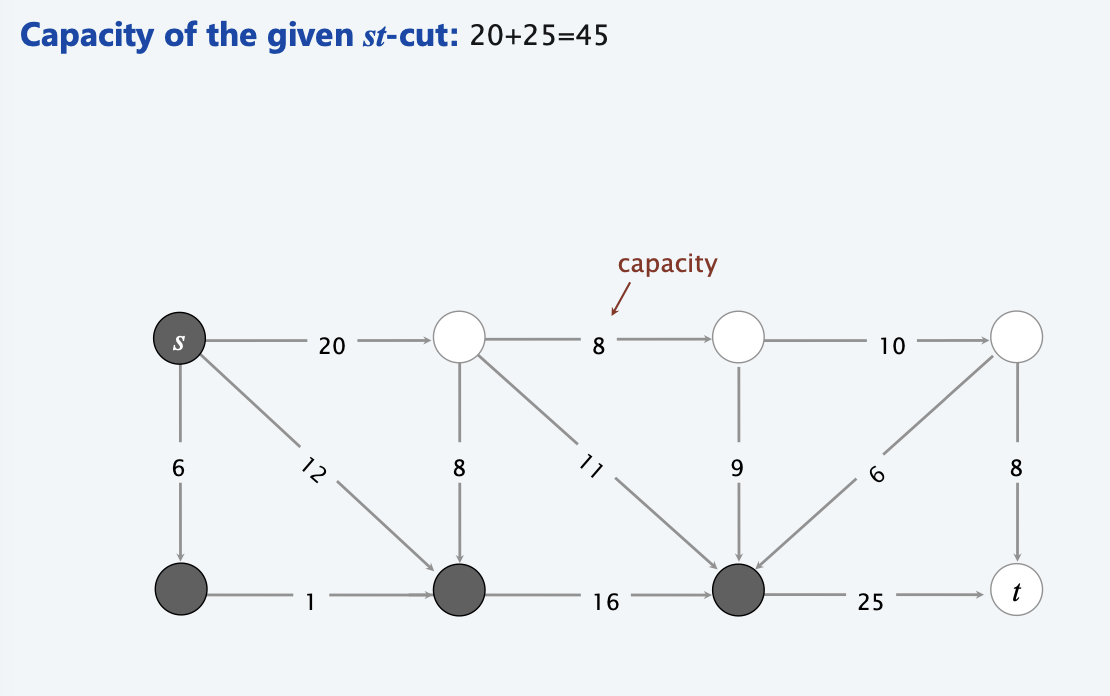
\includegraphics[width=0.5\linewidth]{Screenshot 2024-04-26 alle 10.42.54.png}
    \caption{Capacità di un st-cut}
    \label{fig:enter-label}
\end{figure}
Il problema del Min-cut punta a trovare un cut con capacità minima.\\
Un st-flow(flow) f è una funzione che soddisfa:
\begin{itemize}
    \item Per ogni e$\in$E: $o\leq f(e) \leq c(e)$ (capacity).
    \item Per ogni $v\in V -\{s,t\}$: $\sum_{\mbox{e in to v}}f(e)=\sum_{\mbox{e out of v}}f(e)$ (flow conservation).
\end{itemize}
Il valore del flow f è: $val(f)=\sum_{\mbox{e out of s}}f(e)-\sum_{\mbox{e in to s}}f(e)$.
%Ford-Fulkerson algorithm start
\subsection{Ford-Fulkerson algorithm}
Un algoritmo greedy per il problema del min-cut potrebbe essere:
\begin{itemize}
    \item Inizia con f(e)=0 per ogni e$\in$E.
    \item Trova un path(s,t) P dove ogni arco ha f(e)<c(e).
    \item Aumenta il flow lungo il path P.
    \item Ripeti finchè non rimani bloccato.
\end{itemize}
Questo algoritmo non è corretto perchè una volta che viene incrementato il flow di un arco, questo non viene mai decremenato. 
\begin{figure}
    \centering
    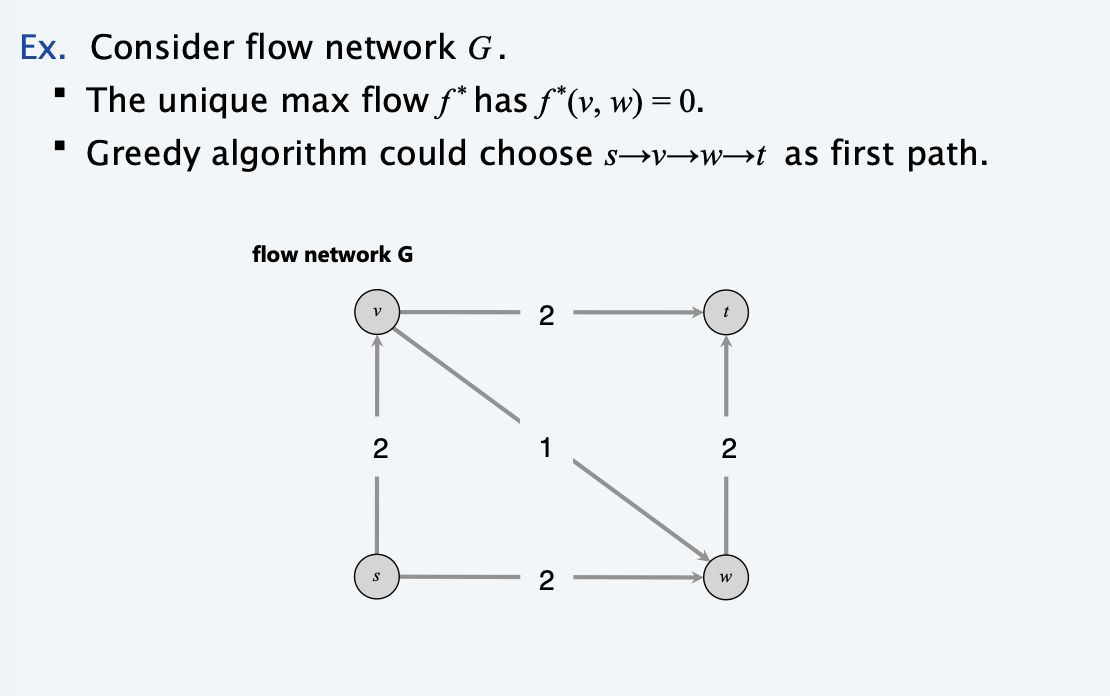
\includegraphics[width=0.5\linewidth]{Screenshot 2024-04-26 alle 10.54.59.png}
    \caption{Greedy algotithm fail}
    \label{fig:enter-label}
\end{figure}
Diamo ora alcune definizioni:\\
Arco originale: e = (u,v)$\in$E, flow f(e), capacity c(e).\\
Arco inverso: $e^{reverse}=(v,u)$, "annulla" il flusso inviato.\\
Capacità residua: \[
c_f(e) =\begin{cases} c(e)-f(e), & \mbox{se }e\in E \\ f(e^{reverse}\in E, & \mbox{se }e^{reverse} \in E
\end{cases}
\]
Rete residua: $G_f=(V,E,s,t,c_f)$. $E_f=\{e:f(e)<c(e)\}\cup\{e:f(e^{reverse})>0\}$.\\ Proprietà chiave: f' è un flow in $G_f$ se f+f' è un flow in G.
\begin{figure}[H]
    \centering
    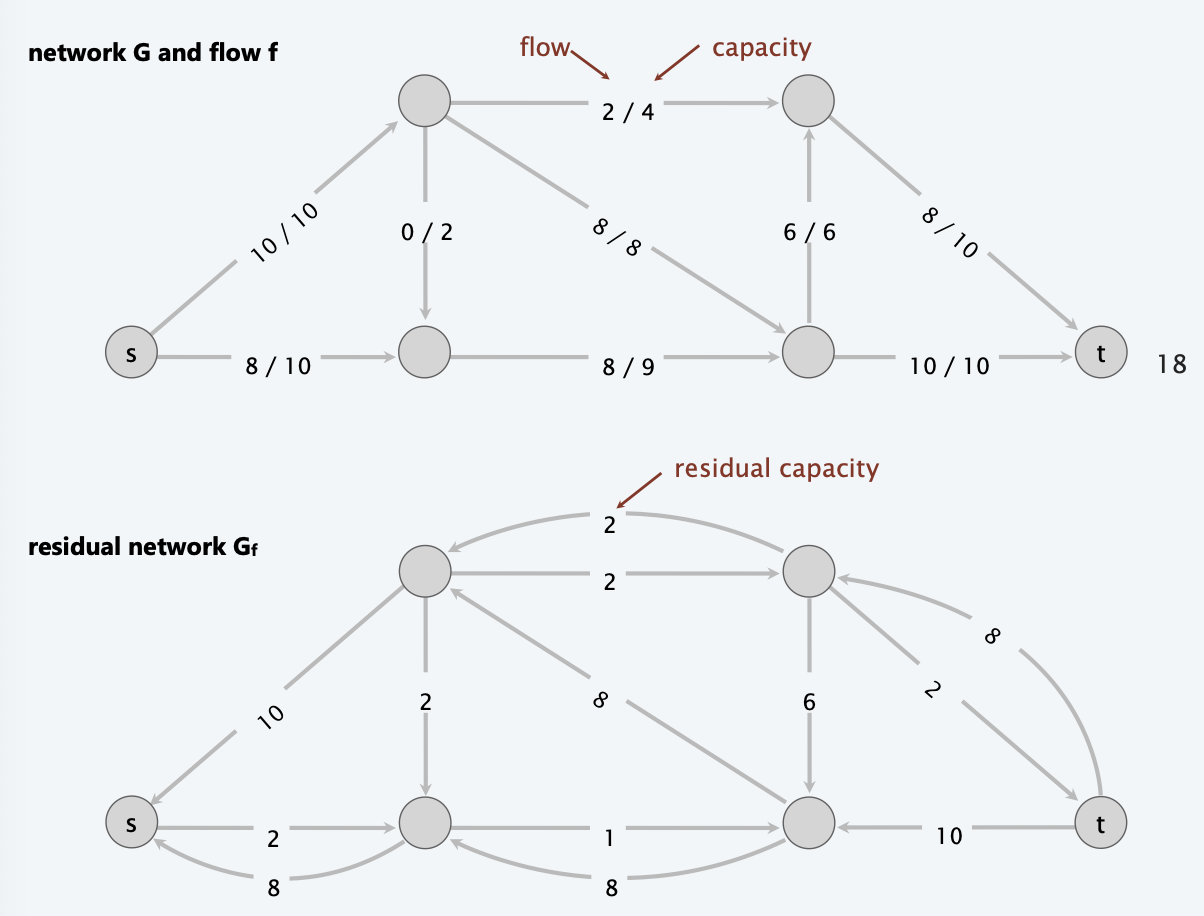
\includegraphics[width=0.5\linewidth]{Screenshot 2024-04-26 alle 11.30.49.png}
    \caption{Esempio residual network}
    \label{fig:enter-label}
\end{figure}
Un augmenting path è un semplica path(s,t) nella rete residua $G_f$.\\
La bottleneck capacityy di un augmenting path P è la capacità minima residua di ogni arco in P.\\
Proprietà chiave: Sia f un flusso e sia P un augmenting path in $G_f$. Allora, dopo la chiamata $f'\leftarrow AUGMENT(f,c,P)$, f' è un flusso e val(f')=val(f)+bottleneck($G_f,P)$.
%%%%%%%%%% algoritmo start 
\begin{center}
\begin{algorithm}
\caption{Augment}
\KwData{$f,c,P$}
$\sigma\leftarrow$ bottleneck capacity dell'augmenting path P\;
\For{arco e$\in$P}{
    \If{e$\in$E}{
       $f(e)\leftarrow f(e) + \sigma\;$
    }
    \Else{$f(e^{reverse})\leftarrow f(e^{reverse})-\sigma\;$}
}
\Return f\;
\end{algorithm}
\end{center}
%%%%%%%%%% algoritmo end
L'algoritmo di Ford-Fulkerson per l'augmenting path:\\
\begin{itemize}
    \item Inizia con f(e)=0 per ogni arco e$\in$E.
    \item Trova un path(s,t) P nella residual network $G_f$.
    \item Augment flow lungo l'arco P.
    \item Ripeti finchè non rimani bloccato
\end{itemize}
\newpage
%%%%%%%%%% algoritmo start 
\begin{center}
\begin{algorithm}
\caption{Ford-Fulkerson}
\KwData{$G$}
\For{arco e$\in$P}{
    f(e)$\leftarrow$0\;
}
$G_f \leftarrow$ residual netword di G rispetto al flusso f\;
\While{esiste un pat P(s,t) in $G_f$}{
    f$\leftarrow$AUGMENT(f,c,P)\;
    Aggiorna $G_f$\;
}
\Return f\;
\end{algorithm}
\end{center}
%%%%%%%%%% algoritmo end
%Ford-Fulkerson algorithm end
%Max-Flow min-cut theorem start
\subsection{Max-Flow min-cut theorem}
\begin{lemma}
    Sia f un qualsiasi flusso e sia (A,B) un qualsiasi cut. Allora il valore del flusso f è uguale al net flow lungo il cut (A,B).\\
    val(f)=$\sum_{\mbox{e out of A}}f(e)-\sum_{\mbox{e in to A}}f(e)$.
\end{lemma}
\begin{proof}
    val(f)=$\sum_{\mbox{e out of s}}f(e)-\sum_{\mbox{e in to s}}f(e)\\=\sum_{v\in A}(\sum_{\mbox{e out of v}}f(e)-\sum_{\mbox{e in to v}}f(e))\\=\sum_{\mbox{e out of A}}f(e)-\sum_{\mbox{e in to A}}f(e)$.
\end{proof}
Proprietà:
\begin{itemize}
    \item Weak duality: Sia f un qualsiasi flusso e (A,B) un qualsiasi cut. Allora, val(f)$\leq$cap(A,B).
    \begin{proof}
        val(f)=$\sum_{\mbox{e out of A}}f(e)-\sum_{\mbox{e in to A}}f(e)\\\leq\sum_{\mbox{e out of A}}f(e)\\\leq\sum_{\mbox{e out of A}}c(e)=cap(A,B)$.
    \end{proof}
    \item Corollario: sia f un flusso e sia (A,B) un qualsiasi cut. Se val(f)=cap(A,B), allora f è un max flow e (A,B) è un min cut.
    \begin{proof}
        Per ogni flusso f': val(f')$\leq$cap(A,B)=val(f).\\
        Per ogni cut(A',B'): cap(A',B')$\geq$val(f)=cap(A,B).
    \end{proof}
\end{itemize}
\begin{theorem}
    Max-Flow min-cut theorem: Il valore del flusso massimo è uguale alla capacità di min cut.\\
    Augmenting path theorem: Un flusso f è un max flow se non ha augmenting paths.
\end{theorem}
\begin{proof}
     Date le seguenti tre condizioni per ogni flusso f:
    \begin{itemize}
        \item Esiste un cut(A,B) tale che cap(A,B)=val(f).
        \item f è un max flow.
        \item Non ci sono augment path rispetto a f
    \end{itemize}
    La prima condizine implica la seconda per il corollario della weak duality.\\
    La seconda condizione implica la terza, lo si può dimostrare ponendo (not(iii) implica not(ii)):
    \begin{proof}
        Supponiamo che esista un augmenting path rispetto a f. Allora possiamo migliorare il flusso f inviando il flusso lungo questo path.  Allora, f non è un max flow.
    \end{proof} 
    La terza condizione implica la prima: Sia f un flusso senza augmenting paths. Sia A un insieme di nodi raggiungibili da s nella rete residua $G_f$. Per definizione di A: $s\in A$. Per definizione del flusso f: $t\notin A$. \\$val(f)=\sum_{\mbox{e out of A}}f(e)-\sum_{\mbox{e in to A}}f(e)\\ =\sum_{\mbox{e out of A}}c(e)-0\\=cap(A,B)$.
\end{proof}
\begin{proof}
    Dato un qualsiasi max flow f, si può calcolare un min cut(A,B) in tempo O(m).
\end{proof}
\begin{proof}
    Sia A un insieme di nodi raggiungibili da s nella rete residua $G_f$.
\begin{figure}[H]
    \centering
    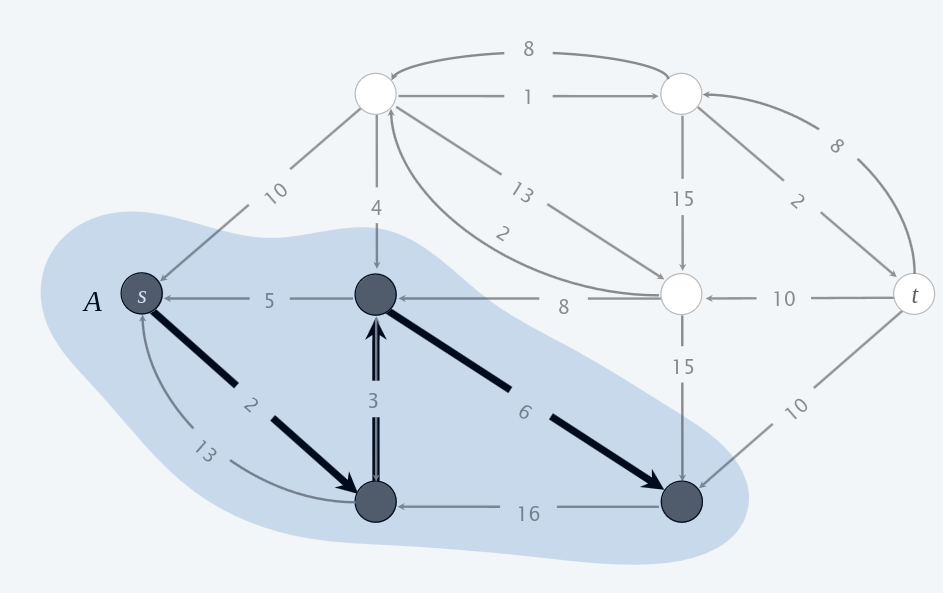
\includegraphics[width=0.5\linewidth]{Screenshot from 2024-04-26 18-51-13.png}
    \caption{Dimostrazione}
    \label{fig:enter-label}
\end{figure}
\end{proof}
Si assuma che ogni arco abbia capacità c(e) intera compresa tra 1 e C.\\
Proprietà Integrality invariant: Attraverso Ford-Fulkerson, ogni arco del flusso f(e) e la capacità residua $c_f(e)$ è un intero. Si può dimostrare per induzione sul numero di augmenting paths.
\begin{theorem}
    Ford–Fulkerson termina dopo al massimo val(f*)$\leq nC$ augmenting paths, dove f* è un max flow.
\end{theorem}
\begin{proof}
    Ogni augmentation aumenta il valore del flusso di almeno 1.
\end{proof}
Corollario: Il running time di questo algoritmo è O(m val(f*))=O(mnC).
\begin{proof}
    Si può usare sia BFS o DFS per trovare un augmenting path in tempo O(m).
\end{proof}
\begin{theorem}
    Esiste un integral max flow f*.
\end{theorem}
\begin{proof}
    Poiché Ford-Fulkerson termina, il teorema segue dall'integrality invariant e augmenting path theorem.
\end{proof}
L'algoritmo FOrd-Fulkerson non ha tempo polimoniale alla grandezza dell'input, è pseudo-polimoniale. Se la capacità massima è C, allora l'algoritmo può fare $\geq$C iterazioni. Il numero di augmenting paths può essere esponenziale all'input size.
%Max-Flow min-cut theorem end
%choosing good augmenting paths start
\subsubsection{Choosing good augmenting paths}
Si può ovviare al problema scegliendo attentamente gli augmenting paths: scegliendo augmenting paths con larga bottleneck capacity si può mantenere un parametro di scaling $\Delta$, Sia $G_f(\Delta)$ la parte del residual network contenente solo archi con capacità $\geq \Delta$. Ogni augmenting path in $G_f(\Delta)$ ha bottleneck capacity $\geq\Delta$.
%%%%%%%%%% algoritmo start 
\begin{center}
\begin{algorithm}
\caption{Capacity-scaling}
\KwData{$G$}
\For{arco e$\in$E}{
    f(e)$\leftarrow$0\;
}
$\Delta\leftarrow \mbox{la più grande potenza di 2}\leq C\;$
\While{$\Delta\geq 1$}{
    $F_f(\Delta)\leftarrow \Delta-\mbox{residual network di G rispetto al flusso f}\;$
    \While{esiste un path P(s,t) in $G_f(\Delta)$}{
    f$\leftarrow$AUGMENT(f,c,P)\;
    Aggiorna $G_f(\Delta)\;$
    }
    $\Delta\leftarrow\delta/2$\;
}
\Return f\;
\end{algorithm}
\end{center}
%%%%%%%%%% algoritmo end
\newpage
Si può dimostrare quanto segue:
\begin{lemma}
    Ci sono 1+$\lfloor \log_2C\rfloor$ fasi di scaling.
\end{lemma}
\begin{lemma}
    Ci sono $\leq 2m$ aumenti per ogni fase di scaling.
\end{lemma}
\begin{theorem}
    Questi due lemmi implicano che il precedente algoritmo costa tempo O($m^2\log C$).
\end{theorem}
Il prossimo augmenting path in Ford-Fulkerson deve essere scelto tra quelli con il minor numero di archi attraverso la BFS.
%%%%%%%%%% algoritmo start 
\begin{center}
\begin{algorithm}
\caption{Shortest-Augmenting-Path}
\KwData{$G$}
\For{arco e$\in$E}{
    $G_f\leftarrow$residual network di G rispetto al flusso f\;
    \While{esiste un path(s,t) in $G_f$}{
    P$\leftarrow$BREADTH-FIRST-SEARCH($G_f$)\;
    f$\leftarrow$AUGMENT(f,c,P)\;
    Aggiorna $G_f$\;
    }
}
\Return f\;
\end{algorithm}
\end{center}
%%%%%%%%%% algoritmo end
Può essere provato quanto segue:
\begin{lemma}
    Il numero totale di aumenti è al massimo mn.
\end{lemma}
\begin{theorem}
    L'algoritmo shortest-augmenting-path costa tempo O($m^2n$).
\end{theorem}
%choosing good augmenting paths end
%bipartite matching start
\newpage
\subsection{Bipartite Matching}
Sia G=(V, E) un grafo non diretto, un sottoinsieme di archi $M\subseteq E$  si dice matching se ogni nodo appare al massimo in un arco M.\\
Il problema del Max Matching consiste nel trovare la cardinalità massima del matching in un dato grafo G.\\
Sia G un grafo, è bipartito se i nodi possono essere partizionati in due sottoinsiemi L e R tale che ogni arco collega un nodo in L con un nodo in R.\\
Il problema del Bipartite matching consiste nel trovare il matching con cardinalità massima di un dato grafo bipartito G=($L\cup R,E$).\\
Dato un grafo G=(V,E), un sottoinsieme di archi $M\subseteq E$ si dice perfect matching se ogni nodo appare esattamente in un arco in M.\\
Perfect matching problem: dato un grafo bipartito G=($L\cup R,E$), trovare un perfect matching o riferire se non esiste.\\
\subsubsection{Bipartite matching: max-flow formulation}
\begin{itemize}
    \item Creare un grafo diretto G'=($L \cup R \cup \{s,t\},E'$).
    \item Direzionare ogni arco da L a R e assegnare capacità infinita.
    \item Aggiungere archi di capacità unitaria da s a ciascun nodo in L.
    \item Aggiungere archi du capacità unitaria da ogni  nodo in R a t.
\end{itemize}
\begin{theorem}
    Esiste una corrispondenza 1-1 tra gli abbinamenti di cardinalità k in G e flussi integrali di valore k in G'.
\end{theorem}
\begin{proof}
 Vedere dimostrazione
\end{proof}
Corollario: Si può risolvere il problema del bipartite matching usando il max-flow formulation. Usando Ford-Fulkerson si hanno $\leq n$augmentations, allora il running time è O(mn).
\begin{proof}
    vedere dimostrazione.
\end{proof}
\begin{figure}[H]
    \centering
    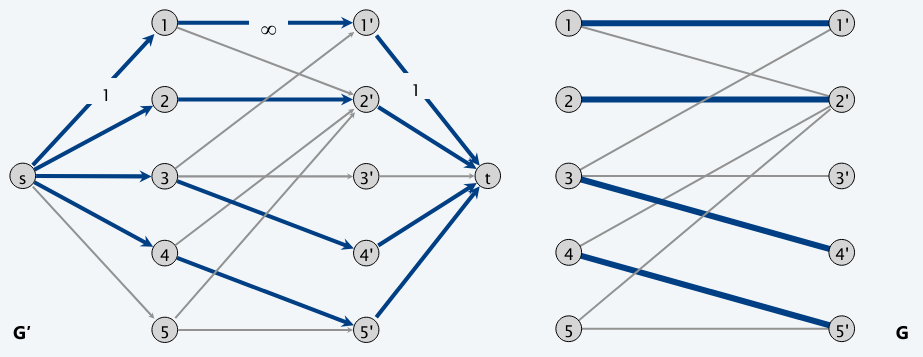
\includegraphics[width=0.5\linewidth]{Screenshot from 2024-05-05 11-22-39.png}
    \caption{Max Flow Formulation}
    \label{fig:enter-label}
\end{figure}
%bipartite matching end
%disjoint paths start
\newpage
\subsubsection{Disjoint paths}
Due percorsi sono edge-disjoint se non hanno archi in comune.\\
Edge-disjoint paths problem: dato un grafo diretto G=(V,E) e due nodi s e t, trovare il numero massimo di edge-disjoint paths(s,t).
\begin{figure}[H]
    \centering
    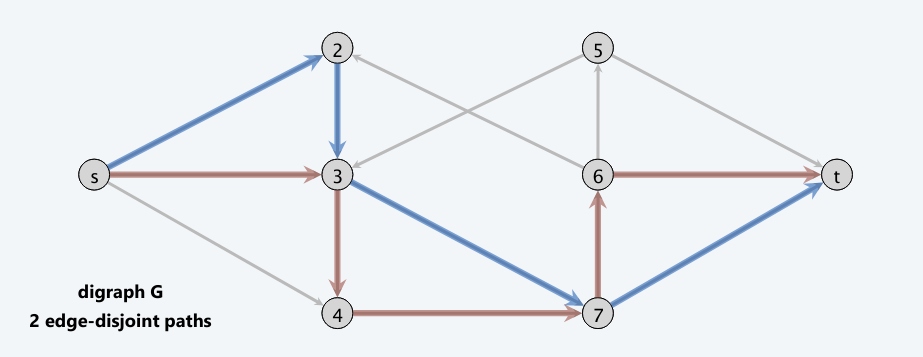
\includegraphics[width=0.5\linewidth]{Screenshot from 2024-05-05 11-29-11.png}
    \caption{Esempio comunication networks}
    \label{fig:enter-label}
\end{figure}
Max-flow formulation: Assegnare un'unità alla capacità di ogni arco.
\begin{theorem}
    Esiste una corrispondenze 1-1 tra k edge-disjoint paths(s,t) in G e integral flow di valore j in G'.
\end{theorem}
\begin{proof}
    dimostrazione
\end{proof}
Corollario: Si può risolvere il problema edge-disjoint paths attraverso la max-flow formulation in tempo O(mn) usando il Ford-Fulkerson con $\leq n$ aumenti.
\begin{proof}
    Dimostrazione
\end{proof}
Edge-disjoint paths problem in undirected graphs: dato un grafo G=(V,E) e due nodi s e t, trovare il numero massimo di edge-disjoint paths(s,t).\\\\
Esercizio\\ \\
%disjoint paths end
%image segmentation start
\newpage
\subsubsection{Image segmentation}
Il problema del image segmentation può essere applicato ad esempio nella divisione delle imagini in regioni coerenti o in generale è un problema centrale nel image processing.\\
\begin{itemize}
    \item Ogni pixel dell'immagine va etichettata come appartenente al primo priano o allo sfondo.
    \item V = insieme di pixel, E = coppie di pixel vicini.
    \item $a_i\leq 0$ la probabilità che il pixel i sia in primo piano.
    \item $b_i\leq 0$ la probabilità che il pixel i sia nello sfondo.
    \item $p_{ij}\leq 0$ è una penalità di separazione per aver etichettato uno dei i e j in primo piano e l'altro come sfondo.
\end{itemize}
Goals:
\begin{itemize}
    \item Accuracy: se $a_i>b_i$ in isolamento(?), preferisci mettere l'etichetta i in primo piano.
    \item Smoothnes: se molti vicini di i sono etichettati in primo piano, dovremmo essere propensi a etichettare i come primo piano.
    \item Trovare la partizione (A,B) che massimizzi:\\ $\sum_{i\in A}a_i+\sum_{j\in B}b_j-\sum_{(i,j)\in E |A\cap\{i,j\}|=1}p_{ij}$
\end{itemize}
Si può formulare come min-cut problem. Massimizzare:\\  $\sum_{i\in A}a_i+\sum_{j\in B}b_j-\sum_{(i,j)\in E |A\cap\{i,j\}|=1}p_{ij}$ \\
è equivalente a minimizzare  $\sum_{j\in B}a_j+\sum_{i\in A}b_i+\sum_{(i,j)\in E |A\cap\{i,j\}|=1}p_{ij}$.\\
Dato un grafo G'=(V',E') dove ogni nodo corrispone ad un pixel. Usare due archi antiparalleli invece di archi non orientati. Aggiungo sorgenti in modo che corrispondano al primo piano. Aggiungo un sink t che corrisponde allo sondo.\\
Consideriamo il mic cut (A,B) in G'. A= primo piano. cap(A,B)=$\sum_{j\in B}a_j+\sum_{i\in A}b_i+\sum_{(i,j)\in E |A\cap\{i,j\}|=1}p_{ij}$, precisamente la quantita che vogliamo minimizzare.
\begin{figure}[H]
    \centering
    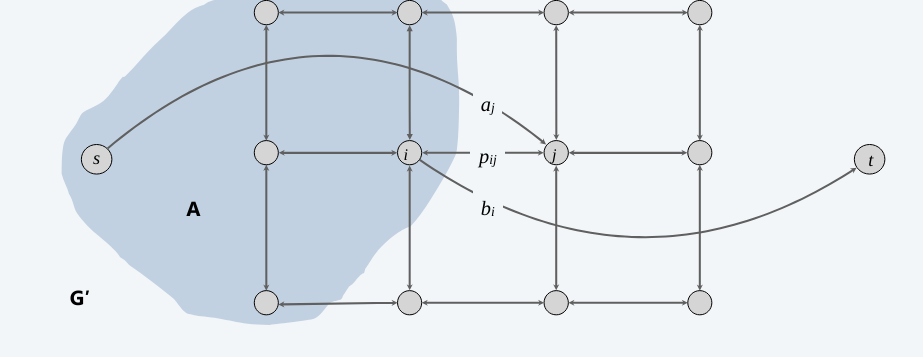
\includegraphics[width=0.5\linewidth]{Screenshot from 2024-05-05 12-15-08.png}
    \caption{Image Segmentation}
    \label{fig:enter-label}
\end{figure}
%image segmentation end
%baseball elimination start
\newpage
\subsubsection{Baseball elimination}
Date delle squadre di baseball trovare il team che ha più probabilità di finire la stagione con più vittorie. La risposta a questa domanda non dipende solo da quante partite hanno già giocato o mancano da giocare, ma anche dall'avversario che avranno contro.\\
Sia S l'insieme delle squadre. Sia z$\in$S una squadra. La squadra x ha vinto $w_x$ partite. La squadra x e la squadra y giocano contro $r_{xy}$ volte aggiuntive. Vista la classifica attuale, ce qualche risultato delle partite rimanenti in cui la squadra z finisce con il maggior numero di punti (o pareggio per la maggior parte) vince?
\begin{figure}[H]
    \centering
    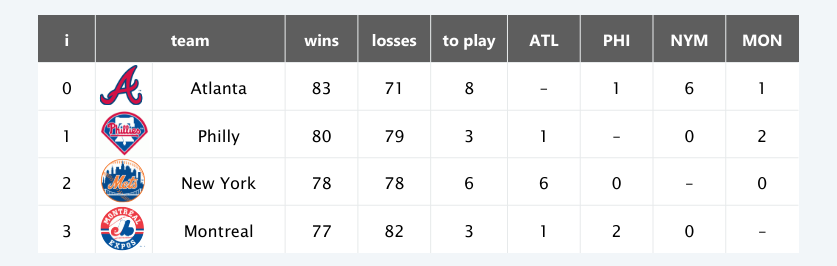
\includegraphics[width=0.5\linewidth]{Screenshot from 2024-05-05 12-28-27.png}
    \caption{Esempio classifica baseball}
    \label{fig:enter-label}
\end{figure}
Assumiamo che il team 4 vinca i rimanenti games, $w_4+r_4$ vittorie.\\
Dividiamo i rimantenti games così da avere gli altri team con $\leq w_4+r_4$ vittorie.
\begin{theorem}
    Il team 4 non eliminata se e solo se il flusso massimo satura tutti i bordi lasciando s.  
\end{theorem}
\begin{proof}
    Integrità del teorema: ogni partita rimanente tra x e y viene aggiunta al numero di vittorie del team x o y. La capacità sugli archi (x,t) garantisce che nessuna squadra vinca troppe partite.
    \begin{figure}[H]
        \centering
        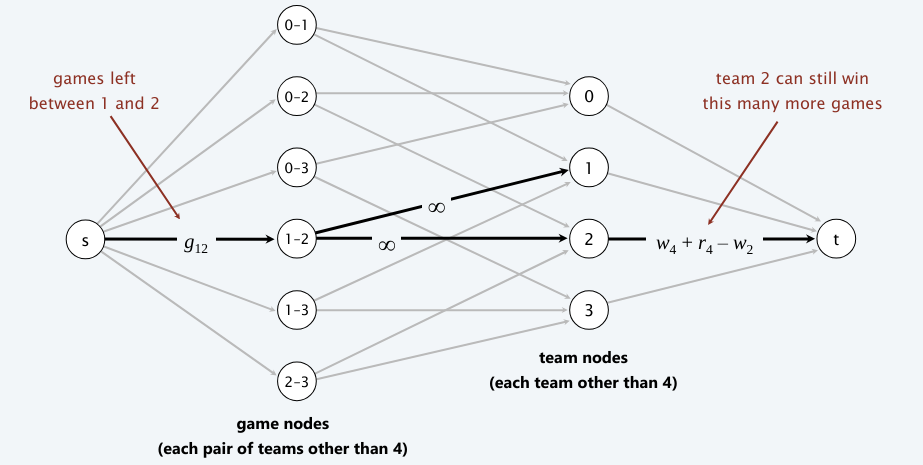
\includegraphics[width=0.5\linewidth]{Screenshot from 2024-05-05 12-26-50.png}
        \caption{Esempio max flow baseball elimination problem}
        \label{fig:enter-label}
    \end{figure}
\end{proof}
%baseball elimination end
%NETWORK FLOW end
%Intractability start
\newpage
\section{Intractability}
%Poly-time reductions start
\subsection{Poly-time reductions}
Algorithm design patterns:
\begin{itemize}
    \item Greedy
    \item Dividi e impere
    \item Programmazione dinamica
    \item Reductions
    \item Duality
    \item Randomization
\end{itemize}
Algoritmh design antipattern:
\begin{itemize}
    \item Np-completezza dice che per alcuni problemi è molto improbabile che ci siano algoritmi polinomiali che li risolvono. 
    \item PSPACE-completeness.
    \item Indecidibile.
\end{itemize}
\noindent Quali problemi possono essere risolti in pratica? Quelli con tempo polinomiale. Un algoritmo con complessità polinomiale si dice robusto per via delle caratteristiche della macchina dove viene eseguito.
A livello pratico un algoritmo polinomiale porta a problemi enormi quando le costanti tendono ad essere grosse.

\noindent Lista problemi che si possono risolvere in tempo polinomiale e non:
\begin{figure}[H]
    \centering
    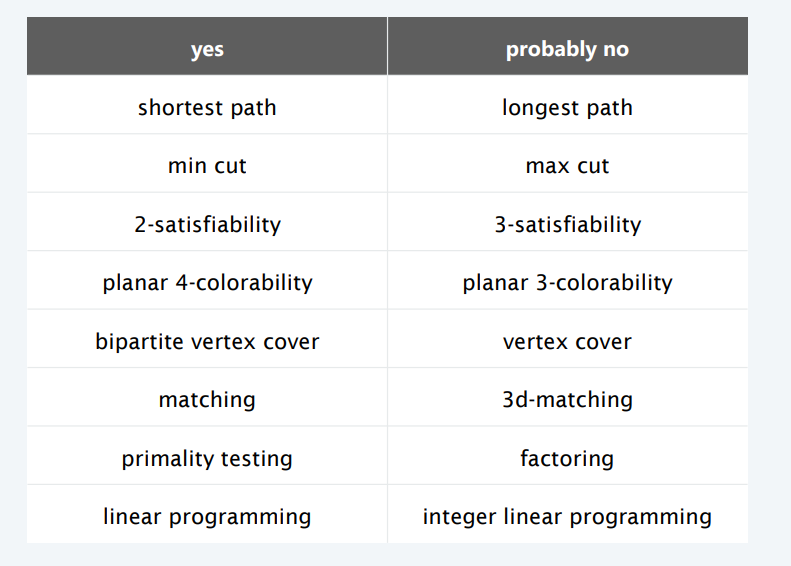
\includegraphics[width=0.5\linewidth]{Screenshot 2024-05-09 120532.png}
    \caption{Problemi polinomiali}
    \label{fig:enter-label}
\end{figure}

\noindent L'idea è quella di catalogare i problemi che si possono risolvere in tempo polinomiale e quelli che non si possono risolvere: 

\noindent Per catalogare questi problemi si usa la riduzione polinomiale (secondo Cook): 
Un problema X si riduce polinomialmente ad un problema Y se posso risolvere X usando un algoritmo polinomiale per Y, si scrive $X \leq_P Y$.
\begin{figure}[H]
    \centering
    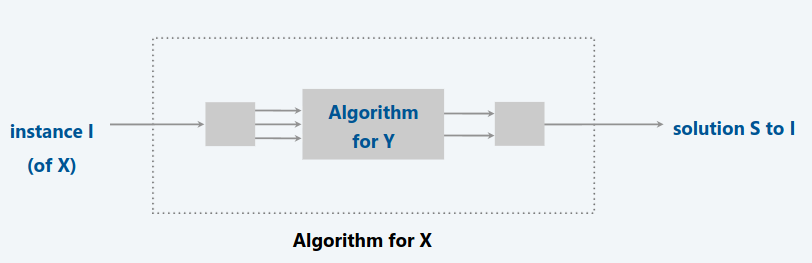
\includegraphics[width=0.5\linewidth]{Screenshot from 2024-05-30 08-27-27.png}
    \caption{Riduzione Polinomiale secondo Cook}
    \label{fig:enter-label}
\end{figure}
\noindent Se $X \leq_P Y$ e Y può essere risolto in tempo polinomiale, allora anche X può essere risolto in tempo polinomiale. 

\noindent Se $X \leq_P Y$ e X non può essere risolto in tempo polinomiale, allora anche Y non può essere risolto in tempo polinomiale. 

\noindent Se $X \leq_P Y$ e $Y \leq_P X$, si scrive $X \equiv_P Y$. In questo caso X può essere risolto in tempo polinomiale se Y può essere risolto in tempo polinomiale.
%Poly-time reductions end
%packing and covering problems start
\newpage
\subsection{Packing and covering problems}
Problema del Indipendent set: 
\begin{itemize}
    \item Dato un grafo G=(V, E) e un intero k, esiste un sottoinsieme di k nodi  che non hanno archi adiacenti?
    \item Vertex-Cover: un vertex-cover è un insieme di vertici che copre tutti gli archi. Dato un grafo G=(V, E) e un intero k, esiste un sottoinsieme di k nodi tale che ogni arco è incidente in almeno uno di quei vertici?
    \item Set-cover: dato un insieme U di elementi, una collezione S di sottoinsieme di U, e un intero k, esistono  $\leq k$ di questi sottoinsiemi la cui unione sia uguale a U?
\end{itemize}
\begin{theorem}
    Independent set $\equiv_P$Vertex-cover.
\end{theorem}
\begin{proof}
    Si deve dimostrare che S è un indipendent set di grandezza k se V-S è un vertex cover di grandezza n-k.
    
    \noindent $\Rightarrow )$ Sia S un qualunque indipendent set di grandezza k. V-S è di grandezza n-k. Sia $(u, v)\in E$. Visto che S è indipendente, allora o $u\notin S$, o $v\notin S$, o entrambi. Così, V-S copre (u, v).

     \noindent $\Leftarrow )$ Sia V-S  un qualsiasi vertex cover di grandezza n-k. S è di grandezza k. Sia $(u, v)\in E$ un arco arbitrario. V-S è n vertex cover, allora o $u\in V-S$, o $v\in V$, o entrambi. Allora o $u \notin S$, o $v \in S$, o entrambi. Quindi S è un insieme indipendente.
\end{proof}
\begin{theorem}
    Vertex-cover $\leq_P$ Set-cover.
\end{theorem}
\begin{proof}
    Prendo un istanza generica di vertex cover e la voglio trasformare in un istanza di set cover.
    \begin{lemma}
        G=(V, E) contiene un vertex cover di grandezza k se(U,S,k) contiene un set cover di grandezza k.
    \end{lemma}
    \begin{proof}
       $\Rightarrow)$Sia X $\subseteq V$ un vertex cover di grandezza k in G. Sia Y=$\{S_v:v\in X\}$  un set cover di grandezza k. Le istanza del vertex cover sono risolte correttamente.
       
       \noindent$\Leftarrow)$Sia $Y\subseteq S$ un set cover di grandezza k in (U,S,k). Sia X =$\{v:S_v\in Y\}$ un vertex cover di grandezza k in G. Le istanze del vertex cover non vengono risolte correttamente.
    \end{proof}
\end{proof}
%packing and covering problems end
%constraint satisfaction problems start
\newpage
\subsection{Constraint satisfaction problems}
Il problema del satisfaction ha le seguenti caratteristiche:
\begin{itemize}
    \item Una variabile booleana o la sua negazione $x_i \mbox{ o } \overline{x_i}$.
    \item Una clausola $C_j=x_1\land \overline{x_2} \land x_3$.
    \item Una formula proposizionale che è una congiunzione di clausole: $\phi=C_1\land C_2 \land C_3 \land C_4$.
    \item Un Sat, data una formula $\phi$ CNF, questa formula è soddisfatta?
    \item 3-Sata un sat dove ogni calusola contiene esattamente 3 letterali e ogni lettera corrisponde a una variabile diversa.
\end{itemize}
\noindent Non esiste un algoritmo con tempo polimoniale per un 3-sat.
\begin{theorem}
    $3-SAT \leq_P Independent-Set$.
\end{theorem}
\begin{proof}
    Data una istanza $\phi$ di un 3-SAT, costruiamo un istanza (G,k) di un indipendent-set che ha un insieme indipendente di dimensione k $\Leftrightarrow \phi$ è soddisfacibile. Costruzione: 
    \begin{figure}[H]
        \centering
        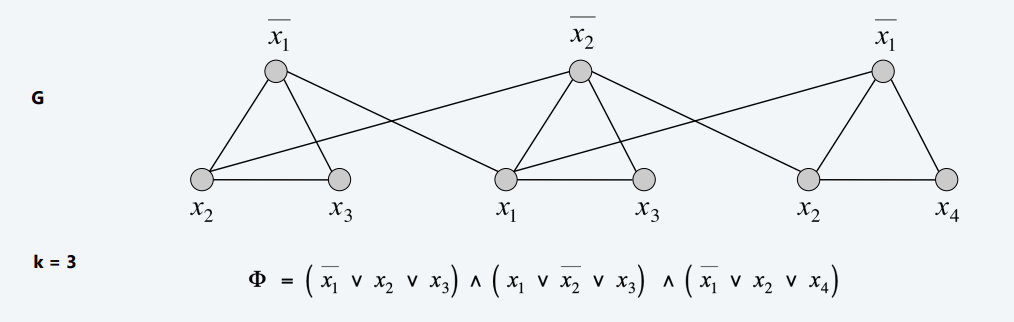
\includegraphics[width=0.5\linewidth]{Screenshot 2024-05-31 171806.png}
        \caption{3-sat}
        \label{fig:enter-label}
    \end{figure}
\end{proof}
\begin{lemma}
    $\phi$ è soddisfacente se e solo se G contiene un insieme indipendente di grandezza k = $|\phi|$.
\end{lemma}
\begin{proof}
   $\Rightarrow)$ Consideriamo una assegnazione che soddisfa $\phi$. Selezioniamo un letterale true per ogni clausola/triangolo. Questo è un indipendent set di grandezza k = $|\phi|$.
   $\Leftarrow)$ Sia S un indipendent set di grandezza k. S può contenere esattamente un nodo per ogni triangolo. Imposta questi valori a true, tutte le clausole in $\phi$ sono soddisfatte.
\end{proof}

\noindent Riepilogo:
\begin{itemize}
    \item Strategie base di riduzione: Indipendent-set $X \equiv_P Y$.
    \item Equivalenza semplice: Vertex-Cover $\leq_P$ Set-Cover.
    \item Da caso speciale a caso generale: 3-SAT $\leq_P$ Indipendent-Set.
\end{itemize}
Proprietà transitiva: Se $X\leq_PY$ e $X \leq_P Z$, allora $X\leq_PZ$.
\begin{figure}[H]
    \centering
    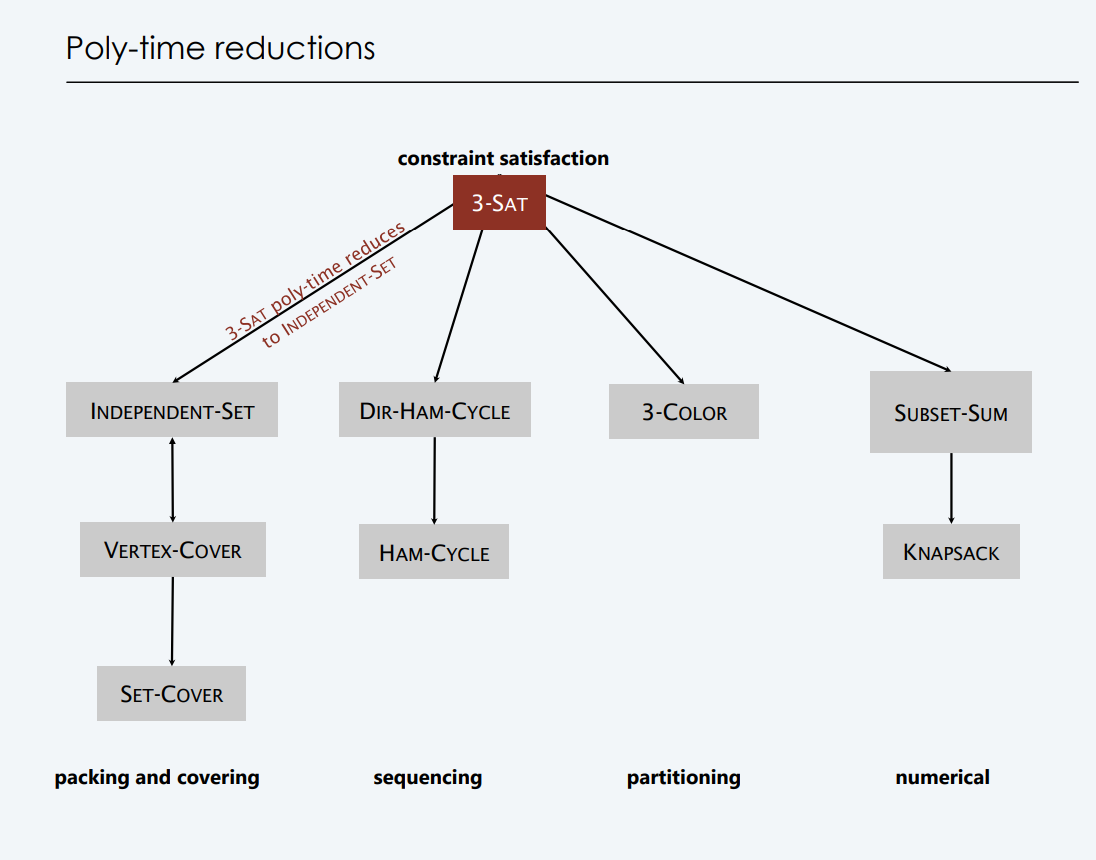
\includegraphics[width=0.5\linewidth]{Screenshot 2024-05-31 190613.png}
    \caption{Poly-Time reduction}
    \label{fig:enter-label}
\end{figure}
%constraint satisfaction problems end
% Problemi a confronto start
\newpage
\subsection{Problemi a confronto}
Tre tipi di problemi:
\begin{itemize}
    \item Decision Problem: Esiste un vertex cover di size $\leq k$?
    \item Search Problem: Trovare un vertex cover di size $\leq k$
    \item Optimization problem: Trovare un vertex cover con size minima.
\end{itemize}
L'obiettivo è  mostrare che tutti e tre i problemi si riducono l'uno all'altro.
\begin{theorem}
    Vertex-cover $\equiv_P$Find-vertex-Cover
    \begin{proof}
        $\leq_P)$Decision probleme è un caso speciale del search problem.

        \noindent $\geq_P)$ Per trovare un vertex cover di grandezza $\leq k$:
        \begin{itemize}
            \item Determino se esiste un vertex cover di grandezza $\leq k$
            \item Trovo un vertice v tale che G - \{v\} è un vertex cover di grandezza $\leq k-1$
            \item  Includo v nel vertex cover.
            \item Ricorsivamente trovo un vertex cover di grandezza $\leq k-1$ in G-\{v\}.
        \end{itemize}     
    \end{proof}
\end{theorem}
\begin{theorem}
     Find-vertex-Cover $\equiv_P$ Find-Min-Vertex-Cover.
     \begin{proof}
           $\leq_P)$Search problem è un caso speciale dell'optimizzation problem.
        \noindent $\geq_P)$ Per trovare un vertex cover di grandezza minima:
        \begin{itemize}
            \item Faccio la ricerca binaria o lineare per la dimensione $k^*$ del min vertex cover.
            \item Risolvo il search problem per $k^*$.
        \end{itemize}  
     \end{proof}
\end{theorem}
% Problemi a confronto end
% P vs NP start
\newpage
\subsection{P vs NP}
Problemi in P:

\noindent Decision Problem: dato un problema X che è un insieme di stringhe. L'istanza s è una sola stringa. Un algoritmo A risolve il problema X: 

\noindent \[
A(s) =\begin{cases}yes, & \mbox{se }s\in X \\ no, & \mbox{se } s \notin X
\end{cases}
\]
Un algoritmo A è di tempo polinomiale se per ogni stringa s, A(s) termina in $\leq p(|s|)$ steps, dove p($\cdot$) è una qualche funzione polinomiale.

\noindent P = insieme dei decision problems per i quali esiste un algoritmo di tempo polinomiale.

\noindent Altri decision problems per i quali esiste un algoritmo con tempo polinomiale:
\begin{figure}[H]
    \centering
    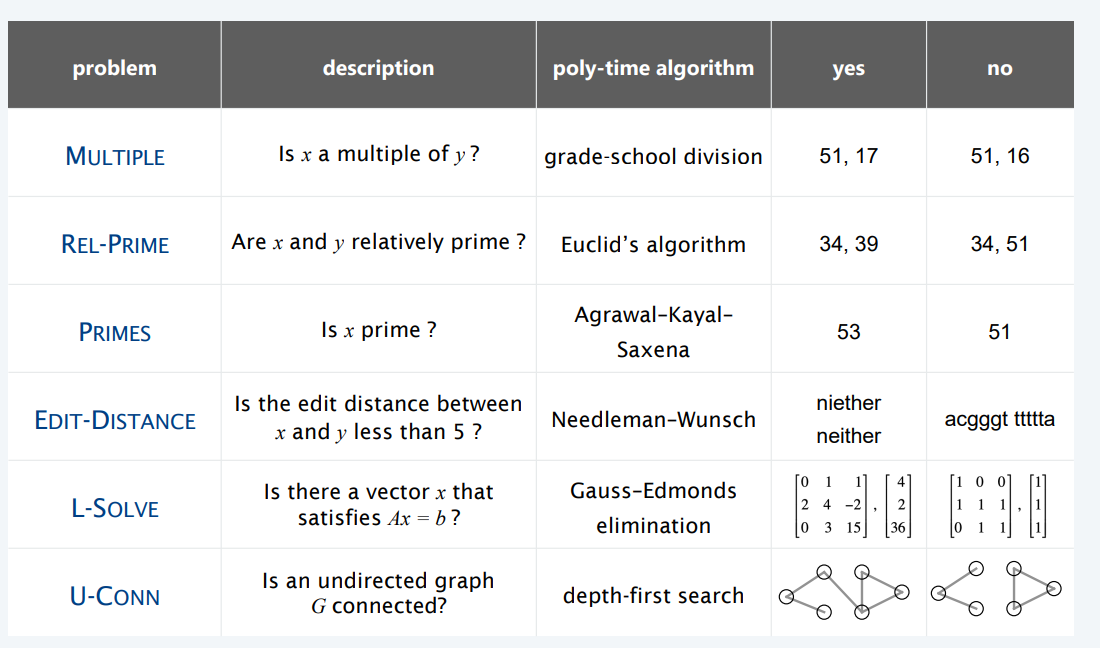
\includegraphics[width=0.5\linewidth]{decisionProblems.png}
    \caption{Decision Problems}
    \label{fig:enter-label}
\end{figure}

\noindent Problemi in NP:

\noindent L'algoritmo C(s, t) è una certificazione per il problema X se per ogni stringa s: s$\in$X se e solo se esiste una stringa t tale che C(s, t)=yes.

\noindent NP = insieme dei decision problems per i quali esiste un algoritmo a tempo polinomiale certificato.

\begin{itemize}
    \item C(s, t) è un algoritmo a tempo polinomiale.
    \item  Il certificato t è di grandezza del polinomio: $|t| \leq p(|s|)$ per ogni polinomio $p(\cdot)$.
\end{itemize}

Problemi decisionali per i quali esiste un certificatore di tempo polinomiale:
\begin{itemize}
    \item Sat, 3-Sat: il certificato è un'assegnazione di valori true alle variabili booleane; Un certificatore verifica che ogni proposizione in $\phi$ abbia almeno un valore letterale true.
    \item Hamilton-Path: Dato un grafo non orientato G=(V, E), esiste un percorso semplice P che visita ogni nodo? Il certificato è una permutazione $\pi$ degli n nodi. Il certificatore verifica che ogni $\pi$ contenga ogni nodo in V esattamente una volta e che G contenga uno spigolo tra ogni coppia di nodi adiacenti.
\end{itemize}
Problemi che probabilmente non appartengono a NP:
\begin{itemize}
    \item Data una posizione sulla scacchiera in una generalizzazione n per n dell pedine, il nero può garantire una vittoria?
    \item Dato un grafo non orientato G=(V,E), la lunghezza del cammino semplice più lungo è $\leq$k?
\end{itemize}
Altri decision problems per i quali esiste un certificato di tempo polinomiale:
\begin{figure}[H]
    \centering
    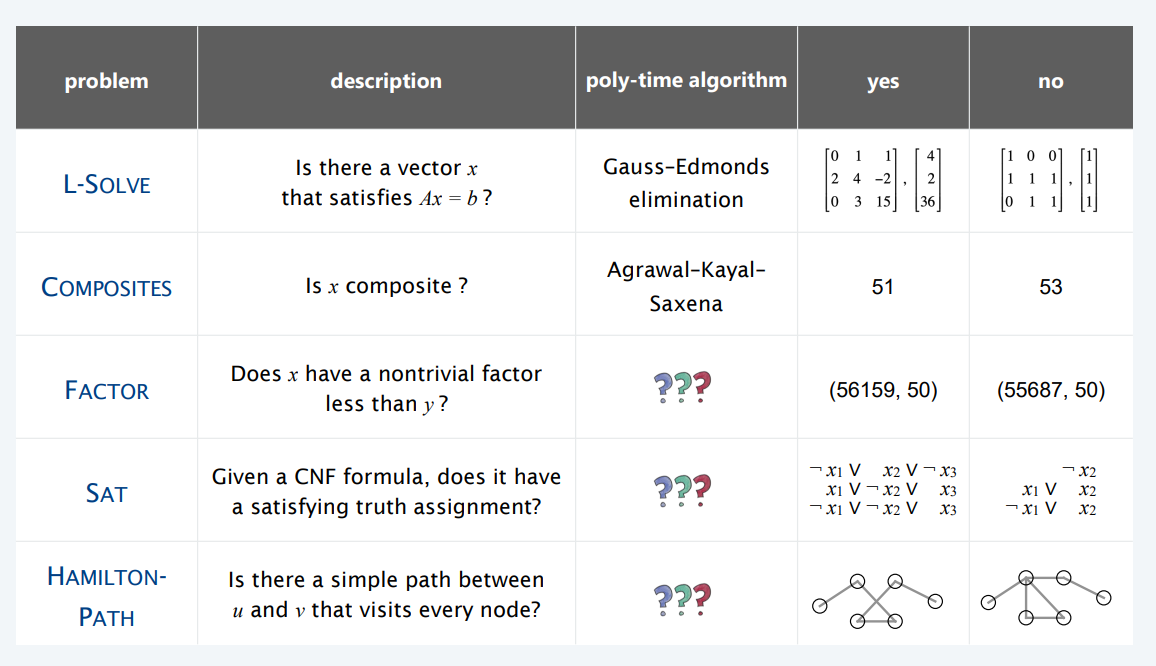
\includegraphics[width=0.5\linewidth]{DecisionProblemsNP.png}
    \caption{NP Decision problems}
    \label{fig:enter-label}
\end{figure}

\begin{lemma}
    $P\subseteq NP$
    \begin{proof}
        Sia $X\in P$ un qualsiasi problema. Per definizione, allora esiste un algoritmo di tempo polinomiale A(s) che risolve X. Un certificato $t=\epsilon$ certifica C(s,t)=A(s).
    \end{proof}
\end{lemma}
\begin{lemma}
    Consideriamo un qualsiasi problema $X\in NP$. Per definizione, esiste un certificatore a tempo polinomiale C(s,t) per X, dove il certificato t soddisfa $|t|\leq p(|s|)$per un qualche polinomio $p(\cdot)$. Per risolvere l'istanza s, eseguo C(s,t) su tutte el stringhe t con $|t|\leq p(|s|)$. Ritorno yes se e solo se C(s,t) ritorna yes per uno qualsiasi di questi certificati.
\end{lemma}
\noindent Fatto: $P\neq EXP \Rightarrow o P\neq NP, o NP\neq EXP, o entrambi$.

\noindent Ancora non c'è una risposta se P = NP, probabilmente no. %%%% Approfondire la questione %%%%%%
% P vs NP end
%NP-complete start
\subsection{NP-complete}
Il problema polinomiale X si riduce (Cook) al problema T se delle istanze arbitrarie di X possono essere risolte usando:
\begin{itemize}
    \item Un numero polinomiale di passi computazionali standard
    \item Un numero polinimiale di chiamate all'oracolo che risolve il problema Y.
\end{itemize}

\noindent Il problema polinomiale X si trasforma (Karp) nel problema Y se data una qualsiasi istanza x di X, possiamo costruire un'istanza y di Y tale che x è un'istanza "yes" di X se e solo se y è un'istanza "yes" di Y.

\noindent Nota: una trasformazione polinomiale è la riduzione polinomiale con solo una chiamata all'oracolo per Y, esattamente alla fine dell'algoritmo per X. Quasi tutte le riduzioni precedenti erano di questa forma.

\noindent Questi due concetti sono gli stessi (abbuso di notazione $\leq_P$) per NP?

\noindent NP-Complete è un problema Y $\in$ NP con la proprietà che per ogni X $\in$ NP, X $\leq_P$Y. 

\noindent Proposizione: Supponiamo che Y $\in$ NP-Complete. Allora, Y $\in$P se e solo se P = NP.
\begin{proof}
    $\Leftarrow)$ Se P = NP, allora Y$\in$P perchè Y$\in$NP.
    $\Rightarrow)$ Supponiamo che Y$\in$P. Consideriamo un qualsiasi problema X$\in$NP. Poiché X$\leq_P$Y, abbiamo x$\in$P. Questo implica che NP$\subseteq$P. Ma conosciamo già P$\subseteq$NP. Così P = NP.
\end{proof}
Un problema "naturale" NP-Completo è il SAT (il primo problema NP-Completo). 

\noindent Per dimostrare che un problema Y è NP-Completo:
\begin{itemize}
    \item Step 1: dimostrare che Y è NP.
    \item  Scegliere un problema X NP-Completo.
    \item Provare che X $\leq_P$Y.
\end{itemize}

\noindent \textbf{Proposizione}: Se X è NP-completo, Y è NP, e X $\leq_P$Y, allora Y è NP-Completo.
\begin{proof}
    Consideriamo un problema W NP. Allora, W $\leq_P$X e X $\leq_P Y$. Per la proprietà transitiva, W $\leq_P$Y. Quindi Y è NP-Completo.
\end{proof}
\noindent Tutti i problemi a cui si riduce il SAT sono NP-Completi.
\noindent La maggior parte dei problemi NP sono noti per essere in P o NP-completi.
\begin{theorem}
    A meno che P = NP, esistono problemi in NP che non sono né in P né NP-Completi.
\end{theorem}
%NP-complete end
%co-NP start
\noindent L'asimmetria di NP: abbiamo bisogno di certificati brevi solo per le istanze "yes".
Esempi:
\begin{itemize}
    \item Sat vs Un-Sat
    \item Hamilton-Cycle vs No-Hamilton-Cycle
\end{itemize}

\noindent Come classificare Un-Sat e No-Hamilton.Cycle? Sat è un NP completo e Sat$\equiv_P$Un-Sat. Hamilton-Cycle è un NP completo e Hamilton-Cycle$\equiv_P$No-Hamilton-Cycle. Ma nè Un-Sat che No-Hamilton-Cycle sono noti per essere in NP.

\noindent Dato un decision problem X, il suo complemento $\overline{X}$ è lo stesso problema con le risposte si e no invertite.

\noindent Si definisce co-NP i complementi dei problemi decisionali in NP.

\noindent Una domanda che resta ancora aperta è NP = co-NP? L'opinione di consenso è no 

\begin{theorem}
    Se NP $\neq$ Co-NP, allora P $\neq$ NP.
    \begin{proof}
        Idea della dimostrazione:
        \begin{itemize}
            \item P è chiuso sotto la complementazione.
            \item Se p = NP, allora NP è chiuso sotto la complementazione.
            \item In altre parole, NP = co-NP.
            \item Questo è il contropositivo del teorema.
        \end{itemize}
    \end{proof}
\end{theorem}
%co-NP end
%Intractability end
%Approximation Algorithms start
\newpage
\section{Approximation Algorithms}
Supponiamo di dover risolvere un problema di ottimizzazione NP-hard. Cosa dovrei fare?

\noindent Bisogna sacrificare una delle tre caratteristiche desiderate, ovvero trovare una soluzione ottima.

\noindent Un p-approximation algorithm è un algoritmo che viene eseguito in tempo polinomiale, risolve istanze arbitrarie del problema e trova una soluzione che rientra nel rapporto p dell'ottimale.

\noindent \textbf{Definizione:} Un algoritmo di $\alpha$-approssimazione per un problema di ottimizzazione è un algoritmo in tempo polinomiale che per tutte le istanze del problema produce una soluzione il cui valore è compreso in un fattore di $\alpha$ il valore di una soluzione ottima.

\noindent $\alpha$ è detto rapporto di approssimazione o fattore di approssimazione.

\noindent Minimization problem:
\begin{itemize}
    \item $\alpha \geq 1$
    \item Per ogni soluzione restituita x, value(x)$\geq\alpha$OPT(x).
\end{itemize}
\noindent Maximization problem:
\begin{itemize}
    \item $\alpha\leq 1$
    \item Per ogni soluzione restituita x, value(x)$\geq\alpha$OPT(x)
\end{itemize}
%Load Balancing start
\subsection{Load Balancing}
Date m macchine identiche, n$\geq$m jobs, il job j viene processato in tempo $t_j$. Il job j deve essere eseguito in modo congiunto su una macchina. Una macchina può processare al massimo un job per volta.

\noindent \textbf{Definizione:} Sia S[i] un sottoinsieme di jobs assegnati alla macchina i. 

\noindent Il carico della macchina i è L[i]= $\sum_{j\in S[i]}t_j$.

\noindent\textbf{Definizione: } Il makespan è il massimo carico su una macchina L=$max_iL[i]$.

\noindent Il problema del \textbf{Load balancing} consiste nell'assegnare ogni job a una macchina per ridurre al minimo il makespan.
\begin{figure}[H]
    \centering
    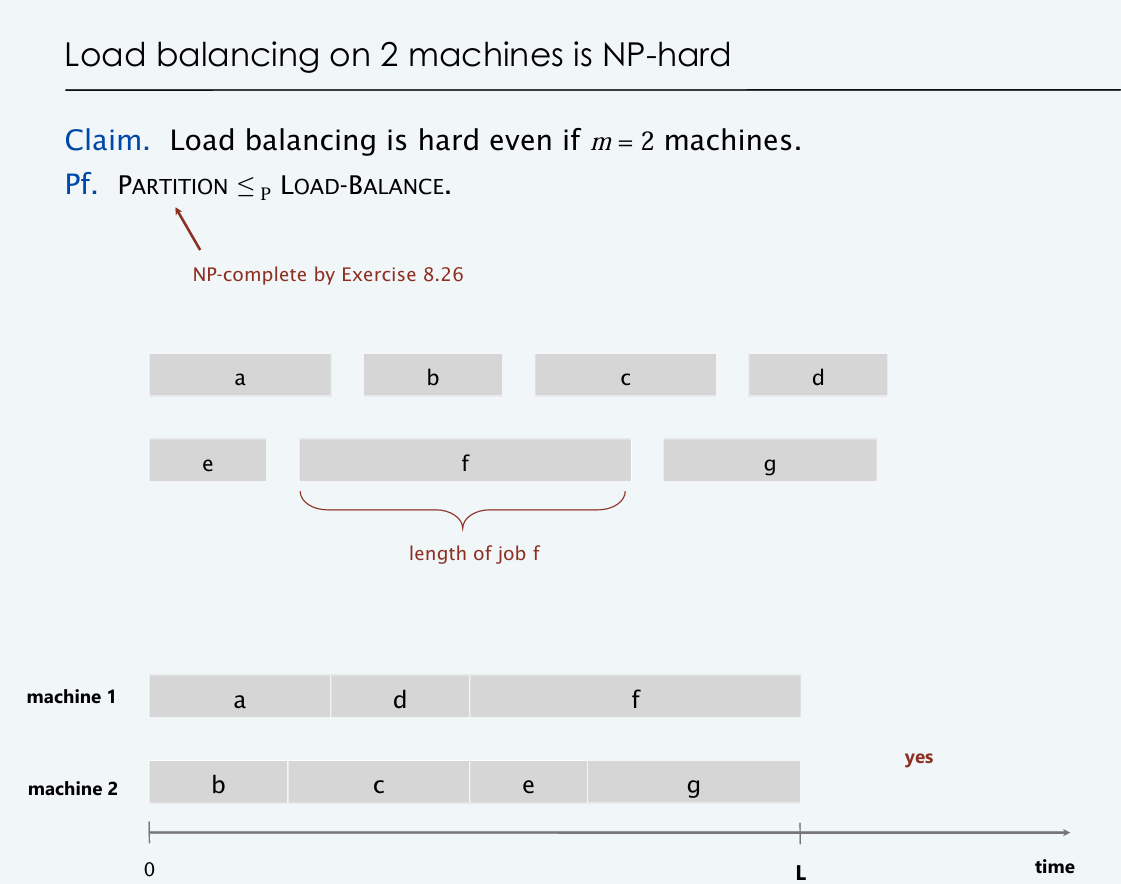
\includegraphics[width=0.5\linewidth]{LoadBalancing_NP-hard.png}
    \caption{Load balancing su 2 macchine}
    \label{fig:enter-label}
\end{figure}
\noindent L'algoritmo per il list-scheduling considera n jobs in un qualche ordine fisso. Assegna il job j alla macchina i il cui carico è più piccolo fino a quel momento.
%%%%%%%%%% algoritmo  start 
\begin{center}
\SetKwComment{Comment}{/* }{ */}
\begin{algorithm}
\caption{algoritmo List-Scheduling}
\KwData{$m, n, t_1, \dots, t_n$}
\KwResult{$S$}
\For{$i = 1$ to $m $}{
   $L[i]\leftarrow0\;$ \Comment{Load on machine i}
   $S[i]\leftarrow\emptyset\;$ \Comment{jobs assigned to machine i}
}
\For{j=1 to n}{
    $i\leftarrow argmin_kL[k]\;$ \Comment{machine i has smallest load}
    $S[i]\leftarrow S[i] \cup \{j\}\;$ \Comment{assign job j to machine i}
    $L[i]\leftarrow L[i]+t_j\;$ \Comment{update load of machine i} 

}
\end{algorithm}
\end{center}
%%%%%%%%%% algoritmo  end
\noindent Questo algoritmo può essere implementato in tempo O($n\log m$) usando una coda di priorità per i carichi L[k].

\begin{lemma}
    Per ogni k: il makespan ottimale è $L^*\geq t_k$.
    \begin{proof}
        Alcune macchine devono elaborare il job che richiede più tempo.
    \end{proof}
\end{lemma}
\begin{lemma}
    Il makespan ottimale è $L^*\geq \frac{1}{m}\sum_kt_k$.
    \begin{proof}
        Il tempo totale di processo è $\sum_kt_k$. Una di m macchine deve fare almeno $\frac{1}{m}$frazioni di lavore totale.
    \end{proof}
\end{lemma}

\begin{theorem}
    L'algoritmo greedy è una 2-approssimazione.
    \begin{itemize}
        \item Prima analisi del caso peggiore di un algoritmo di approssimazione.
        \item Necessita di confrontare la soluzione risultante con il makespan ottimale $L^*$.
    \end{itemize}
    \begin{proof}
    Consideriamo i carichi L[i] della macchina i con il collo di bottiglia (quella che termina con il carico più alto). Sia j l'ultimo job schedulato nella macchina i. Quando il job j viene assegnato alla macchina i, i aveva il carico più piccolo.
    Il suo carico prima dell'assegnazione è $L[i]-t_j$; quindi $L[i]-t_j\leq L[k] \forall 1\leq k \leq m$. 

    \noindent Sommando le disuguaglianze su tutti i k e dividendo per m:
    \begin{center}
        $$
        L[i]-t_j \leq \frac{1}{m}\sum_kL[k] = \frac{1}{m}\sum_kt_k \leq L^*.    
        $$
    \end{center}  
    Adesso, $L = L[i] = \underbrace{(L[i]-t_j)}_\text{per la disuguaglianza sopra $\leq L^*$}+\underbrace{t_j}_\text{per il lemma 1 $\leq L^*$} \leq 2L^*$
    \end{proof}
\end{theorem}

%%%%%%%%%% algoritmo  start 
\begin{center}
\SetKwComment{Comment}{/* }{ */}
\begin{algorithm}
\caption{LPT-List-Scheduling}
\KwData{$m, n, t_1, \dots, t_n$}
\KwResult{$S$}
Ordina i jobs e renumerali in modo che $t_1\geq t_2 \geq\dots\geq t_n\;$
\For{i = 1 to m }{
   $L[i]\leftarrow0\;$ \Comment{Load on machine i}
   $S[i]\leftarrow\emptyset\;$ \Comment{jobs assigned to machine i}
}
\For{j=1 to n}{
    $i\leftarrow argmin_kL[k]\;$ \Comment{machine i has smallest load}
    $S[i]\leftarrow S[i] \cup \{j\}\;$ \Comment{assign job j to machine i}
    $L[i]\leftarrow L[i]+t_j\;$ \Comment{update load of machine i} 

}
\end{algorithm}
\end{center}
%%%%%%%%%% algoritmo  end
\noindent\textbf{Osservazione:} Se la macchina i con il collo di bottiglia ha un solo job, allora è ottimo.
\begin{proof}
    Qualsiasi soluzione deve pianificare tale processo.
\end{proof}
\begin{lemma}
    Se ci sono più di m jobs, $L^*\geq 2t_{m+1}$.
    \begin{proof}
        Consideriamo i tempi di elaborazione dei primi m+1 jobs $t_1\geq t_2\geq\dots\geq t_{m+1}$. Ognuno richiede almeno tempo $t_{m+1}$. Ci sono m+1 jobs e m macchine, quindi per il principio pigeonhole, almeno una macchina ha 2 jobs.
    \end{proof}
\end{lemma}
\begin{theorem}
    La regola LPT è un algoritmo 3/2-approximation.
    \begin{proof}
        Consideriamo il carico l[i] della macchina i con il collo di bottiglia. Sia j l'ultimo job schedulato nella macchina i. Allora,
        \begin{center}
            $$
             L = L[i] = \underbrace{(L[i]-t_j)}_\text{per la disuguaglianza sopra $\leq L^*$}+\underbrace{t_j}_\text{per il lemma 3 $\leq \frac{1}{2}L^*$} \leq \frac{3}{2}L^*
            $$
        \end{center}
    \end{proof}
\end{theorem}
Questa non è un'analisi stretta, a differenza dell'analisi di Graham:
\begin{theorem}
    La regola LPT è una 4/3-approximation.
    \begin{proof}
        Analisi più approfondita dello stesso algoritmo.
    \end{proof}
\end{theorem}
%Load Balancing end
%Center selection start
\newpage
\subsection{Center Selection}
Presi in input n siti $s_1, \dots, s_n$ e un intero k > 0. Il Center Selection problem consiste nel selezionare k centri C tali che la distanza massima tra un sito ed il centro più vicino sia minimizzata. (Una variante aggiunge un vincolo, ovvere che i centri devono corrispondere ad un sito)
\begin{figure}[H]
    \centering
    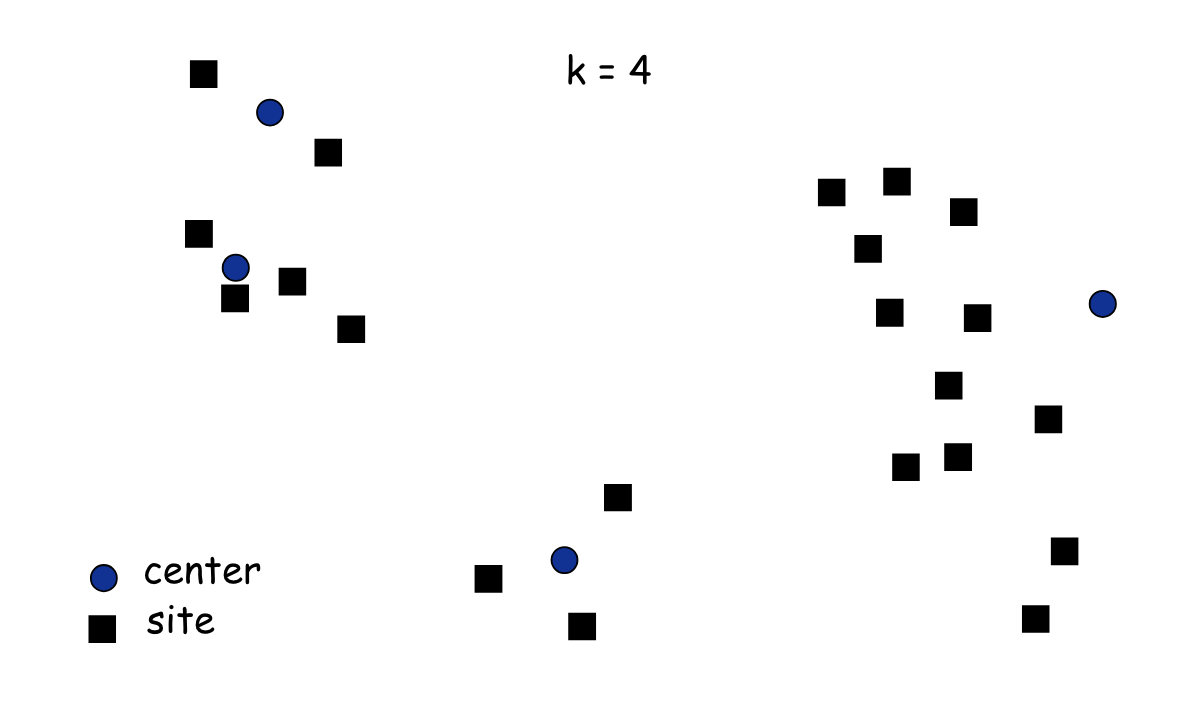
\includegraphics[width=0.5\linewidth]{SelectionCenter.png}
    \caption{Center selection problem}
    \label{fig:enter-label}
\end{figure}
\noindent\textbf{Notazioni:} 
\begin{itemize}
    \item dist(x, y) = distanza tra x e y
    \item dist($s_i, C$)= $min_{c\in C}dist(s_i,c)$= distanza da $s_i$ al centro più vicino.
    \item r(C)= $max_i dist(s_i, C)$= il più piccolo raggio di copertura.
\end{itemize}

\noindent L'obiettivo è trovare un insieme di centri C che minimizzano r(C) di cardinalità k.

\noindent \textbf{Alcune Propietà:}
\begin{itemize}
    \item dist(x, x) = 0, detta identità;
    \item dist(x, y) = dist(y, x), detta simmetria;
    \item dist(x, y) $\leq$ dist(x,z) + dist(z,y), detta disiguaglianza triangolare.
\end{itemize}

\noindent Ecco un algoritmo greedy che seglie ripetutamente il centro successivo come sito più lontano da qualsiasi centro esistente:

\newpage
%%%%%%%%%% algoritmo  start 
\begin{center}
\begin{algorithm}
\caption{Greedy-Center-Selection}
\KwData{$k, n, s_1, \dots, s_n$}
\KwResult{C}
$C=\emptyset$\;
\For{i = 1 to k }{
   Seleziona un sito $s_i$ con distanza massima $dist(s_i, C)$\;
   aggiungi $s_i$ a C\;
}
\Return C;
\end{algorithm}
\end{center}
%%%%%%%%%% algoritmo  end

\noindent\textbf{Osservazione:} Al termine tutti i centri in C sono separati almendo da r(C) coppie. La dimostrazione è data dalla costruzione dell'algoritmo.
\begin{theorem}
    Sia $C^*$ un insieme ottimale di centri. Allora $r(C)\leq 2r(C^*)$.
    \begin{proof}
        \textbf{Per assurdo:} sia $r(C^*)<\frac{1}{2}r(C)$.

        \noindent Per ogni sito $c_i$ in C, consideriamo dei cerchi di raggio $\frac{1}{2}r(C)$ intorno ad essi.
        I cerchi sono disiunti poiché tutti i centri in C sono a coppie a distanza almeno r(C) e c'è esattamente un $c_i^*$ in ogni cerchio.  Ogni cerchio con un centro $c_i\in C$ deve contenere un centro in $C^*$ (altrimenti $dist(c_i,C^*)\geq\frac{1}{2}r(C)>r(C^*))$; I cerchi sono disgiunti e $|C|=|C^*|$.

        \noindent Per ogni sito $c_i$ in C, si consideri un cerchio di raggio $\frac{1}{2}r(C)$ attorno ad esso. Esattamente un $c_i^*$ in ogni cerchio; Sia $c_i$ il sito abbinato a $c_i^*$. Si consideri qualsiasi sito s e il suo centro più vicino $c_i^*$ in $C^*$. 

           $$dist(s, C)\leq 
 dist(s,c_i) \underbrace{\leq}_{\delta\text{-disiguaglianza}}$$\\
$$ \underbrace{dist(s,c_i^*) + dist(c_i^*,c_i)}_{\leq r(C^*)\text{ poiché }c_i^* \text{ è il centro più vicino}} \leq$$ \\
 $$ leq 2r(C^*).$$
 Quindi $r(C) \leq 2r(C^*)$.
    \end{proof}
\end{theorem}
\begin{theorem}
    L'algoritmo greedy mostrato è una 2-approssimazione per il problema di selezione del centro.
    
    \noindent \textbf{Osservazione: } Questo algoritmo posizione sempre i centri nei siti, ma è ancora all'interno di un dattore di 2 della soluzione migliore che consente di posizionare i centri ovunque.
\end{theorem}
\noindent E' molto improbabile che si possa migliorare questa approssimazione
\begin{theorem}
    A meno che P = NP, non esiste $\rho$-approssimazione per il problema del center-selection per ogni $\rho<2.$
\end{theorem}
%Center selection end
%Approximation Algorithms end
\end{document}
%document end